\documentclass[11pt]{article}
\usepackage[T1]{fontenc}
\usepackage{lmodern}
\input{glyphtounicode}
\pdfgentounicode=1
\pdfglyphtounicode{parenleftbig}{0028}
\pdfglyphtounicode{parenrightbig}{0029}
\pdfglyphtounicode{vextendsingle}{23D0}
\pdfglyphtounicode{parenleftBig}{0028}
\pdfglyphtounicode{parenrightBig}{0029}
\pdfglyphtounicode{parenleftbigg}{0028}
\pdfglyphtounicode{parenrightbigg}{0029}
\pdfglyphtounicode{parenleftBigg}{0028}
\pdfglyphtounicode{parenrightBigg}{0029}
\pdfglyphtounicode{braceleftBigg}{007B}
\pdfglyphtounicode{bracerightBigg}{007D}
\pdfglyphtounicode{parenlefttp}{239B}
\pdfglyphtounicode{parenrighttp}{239E}
\pdfglyphtounicode{parenleftbt}{239D}
\pdfglyphtounicode{parenrightbt}{23A0}
\pdfglyphtounicode{summationtext}{2211}
\pdfglyphtounicode{integraltext}{222B}
\pdfglyphtounicode{uniontext}{22C3}
\pdfglyphtounicode{summationdisplay}{2211}
\pdfglyphtounicode{integraldisplay}{222B}
\pdfglyphtounicode{uniondisplay}{22C3}
\pdfglyphtounicode{hatwide}{0302}
\pdfglyphtounicode{hatwider}{0302}
\pdfglyphtounicode{tildewide}{0303}
\usepackage[margin=1in]{geometry}
\usepackage{amsmath,amssymb,amsthm,mathtools,mathrsfs}
\usepackage{microtype}
\usepackage{graphicx,xcolor,tikz}
\usetikzlibrary{arrows.meta,calc,patterns,positioning}
\usepackage{enumitem}
\usepackage{hyperref}
\hypersetup{colorlinks=true,linkcolor=blue!45!black,citecolor=blue!45!black,
  urlcolor=blue!45!black,pdftitle={Global Spherical Shells on Minimal Surfaces of Class VII},
  pdfauthor={OpenAI},pdfsubject={Complex surfaces and the Global Spherical Shell conjecture}}
\numberwithin{equation}{section}
\newtheorem{theorem}{Theorem}[section]
\newtheorem{lemma}[theorem]{Lemma}
\newtheorem{proposition}[theorem]{Proposition}
\newtheorem{corollary}[theorem]{Corollary}
\theoremstyle{definition}
\newtheorem{definition}[theorem]{Definition}
\theoremstyle{remark}
\newtheorem{remark}[theorem]{Remark}
\newcommand{\CC}{\mathbb C}
\newcommand{\RR}{\mathbb R}
\newcommand{\ZZ}{\mathbb Z}
\newcommand{\NN}{\mathbb N}
\newcommand{\PP}{\mathbb P}
\newcommand{\OO}{\mathcal O}
\newcommand{\KK}{K}
\newcommand{\dbar}{\bar\partial}
\newcommand{\ddc}{dd^c}
\newcommand{\eps}{\varepsilon}
\DeclareMathOperator{\supp}{supp}
\DeclareMathOperator{\rank}{rank}
\DeclareMathOperator{\ind}{ind}
\DeclareMathOperator{\Area}{Area}
\DeclareMathOperator{\Mass}{Mass}
\DeclareMathOperator{\coker}{coker}
\DeclareMathOperator{\dist}{dist}
\setlist{itemsep=3pt,topsep=5pt}
\title{Global Spherical Shells on Minimal Surfaces of Class VII}
\author{OpenAI}
\date{September 24, 2026}

\begin{document}
\maketitle

\begin{abstract}
We prove the Global Spherical Shell conjecture: every connected minimal
compact complex surface of class VII with positive second Betti number
contains a global spherical shell. This is a holomorphically embedded
neighborhood of the standard three-sphere in $\CC^2\setminus\{0\}$
whose complement is connected.
\end{abstract}

\section{Introduction}

A compact complex surface is of \emph{class VII} if its first Betti
number is one and its Kodaira dimension is $-\infty$. The classification
of these non-K\"ahler surfaces divides according to the second Betti
number. In the minimal case with $b_2=0$, work of Bogomolov,
Li--Yau--Zheng, and Teleman leads to the classification by Hopf and
Inoue surfaces \cite{Bogomolov1976,LiYauZheng1994,Teleman1994}.
The positive-$b_2$ case is the setting of the Global Spherical Shell
conjecture.

A \emph{global spherical shell} in a complex surface is a holomorphically
embedded neighborhood of the unit three-sphere in $\CC^2\setminus\{0\}$
whose complement is connected. Kato introduced this structure
\cite{Kato1977}. Nakamura's classification program includes the
conjecture that every minimal class VII surface with positive second
Betti number contains such a shell
\cite[Working Hypothesis~5.5]{Nakamura1984}; see also
\cite{Nakamura1989,Teleman2010}. We prove this assertion.

\begin{theorem}[Global Spherical Shell conjecture]\label{thm:main}
Let $X$ be a connected compact complex surface with
\[
 b_1(X)=1,\qquad b_2(X)>0,\qquad \kappa(X)=-\infty.
\]
Assume that $X$ is minimal: it contains no smooth rational curve of
self-intersection $-1$. Then there are an open neighborhood $U$ of
\[
 S^3=\{z\in\CC^2:|z|=1\}
 \quad\text{in }\CC^2\setminus\{0\},
\]
an open subset $\Sigma\subset X$, and a biholomorphism
$\phi:U\longrightarrow\Sigma$ such that $X\setminus\Sigma$ is connected.
\end{theorem}

Kato's deformation theorem then identifies the deformation behavior and
smooth topology of every surface in this range. A primary Hopf surface
is a compact quotient of $\CC^2\setminus\{0\}$ by the infinite cyclic
group generated by a holomorphic contraction.

\begin{corollary}[Deformation and smooth topology]\label{cor:topology}
Let $X$ satisfy the hypotheses of Theorem~\ref{thm:main}, and put
$b=b_2(X)$. There is a small one-parameter deformation
$\mathcal X\to\Delta$ over a disk about $0$, with $\mathcal X_0\simeq X$,
such that every nonzero fiber is obtained from a primary Hopf surface by
exactly $b$ successive point blowups. The centers may be infinitely near.
Moreover,
\[
 \pi_1(X)\cong\ZZ,\qquad
 X\cong_{\mathrm{or}}(S^1\times S^3)\#\,b\,\overline{\mathbb{CP}}^{\,2},
\]
where the second is an orientation-preserving diffeomorphism for the
complex orientation of $X$.
\end{corollary}

The theorem also removes the possible class VII exception in the
geography of aspherical complex surfaces studied by
Albanese--Di Cerbo--Lombardi \cite{AlbaneseDiCerboLombardi2025}.
Here asphericity means that the topological universal cover is
contractible.

\begin{corollary}[A sharpened Euler--signature inequality]
\label{cor:aspherical-geography}
Let $S$ be a connected closed smooth complex surface whose topological
universal cover is contractible. Write $\chi_{\mathrm{top}}(S)$ for its
Euler characteristic and $\sigma(S)$ for its signature in the complex
orientation. Then
\[
 \chi_{\mathrm{top}}(S)\geq\frac95|\sigma(S)|.
\]
If $\chi_{\mathrm{top}}(S)>0$, then $S$ is of general type; otherwise
$\chi_{\mathrm{top}}(S)=\sigma(S)=0$.
\end{corollary}

The proofs of these consequences are given in
Section~\ref{sec:consequences}. We turn to the geometric reductions and
the analytic construction that prove the main theorem.

\subsection*{Curves, shells, and earlier approaches}

The shell construction makes the positive-$b_2$ classification problem
concrete: one modifies a ball and glues its boundary neighborhoods by a
holomorphic embedding. Kato introduced the shell framework
\cite{Kato1977}; Dloussky developed its description by sequences of
blowups and contracting germs \cite{Dloussky1984}. The conjecture asks
whether an arbitrary minimal class VII surface with positive second
Betti number admits this geometry, even when no curves are initially
known to exist.

Two curve criteria reduce the task. Enoki's theorem handles the
presence of a nonzero effective divisor of square zero
\cite{Enoki1981}. In the remaining case, Dloussky, Oeljeklaus, and
Toma prove that $b_2(X)$ rational curves imply a global spherical shell
\cite{DOT2003}. Throughout this paper a rational curve may be singular:
its normalization is $\PP^1$. These criteria shift the burden to
producing sufficiently many rational curves on a surface whose
intersection form is negative definite. A topological cohomology class
alone does not provide an effective divisor, and an effective divisor
on a noncompact cover need not have compact components.

Gauge theory has supplied major advances in this curve-production
problem. Teleman proved the shell conjecture for $b_2=1$ and proved
that a minimal class VII surface with $b_2=2$ contains a cycle of
curves \cite{Teleman2005,Teleman2010}. The cycle conclusion is distinct
from the general criterion requiring $b_2$ rational curves.
Dloussky's numerically anticanonical and later twisted-logarithmic-form
criteria give further routes from additional geometric structure to a
shell \cite{Dloussky2006,Dloussky2025}. Kurnosov and Spicer obtain the
shell conclusion for $b_2=3$ when two distinct singular holomorphic
foliations are present \cite{KurnosovSpicer2026}.

Infinite divisors on covers also occur in the deformation work of
Dloussky and Teleman \cite{DlousskyTeleman2012}. For families of
surfaces with shells, they describe lifted exceptional divisors whose
limits can be infinite sums of compact curves. Their extension theorem
for more general degenerations still supplies effective divisors, but
leaves open whether open Riemann surfaces can occur as components.
This distinction is central here. We construct divisors directly on
the infinite cyclic cover of the given surface, and prove that every
component is compact. The estimates must work for all the compact
Chern classes needed in the eventual curve count.

The weighted analysis uses the Fourier--Laplace method for periodic
ends developed by Taubes \cite{Taubes1987}; the treatment of elliptic
complexes by Mrowka--Ruberman--Saveliev \cite{MRS2014} provides a
related framework. We prove the Dolbeault statements needed here from
acyclicity of compact character bundles, including the continuation
through the trivial character. For compactness of curve components,
the argument combines residue currents, analytic-cycle compactness
\cite{Bishop1964,HarveyShiffman1974}, and Fourier estimates on source
cylinders. A periodic gauge estimate uses exponential integrability
\cite{Trudinger1967} to control the remaining plane case.

\subsection*{The argument}

After Enoki's reduction we assume that no nonzero effective divisor
has square zero. Let $Y\to X$ be the infinite cyclic cover associated
with a primitive integral class in $H^1(X;\ZZ)$, and let $T$ generate
its deck group. We choose a proper height $h$ satisfying
$h\circ T=h+1$, with positive constant complex Laplacian for a lifted
Gauduchon metric. The positive and negative ends mean $h\to+\infty$
and $h\to-\infty$, respectively. Write $K_Y$ for the canonical bundle
and also for its first Chern class in intersection products.

\paragraph{Compact classes and holomorphic sections.}
A compact line-bundle datum is a smooth line bundle $E\to Y$ with
specified trivializations outside a compact set. Those trivializations
define a relative Chern class $e\in H_c^2(Y;\ZZ)$. The finite cyclic
quotient $X_n=Y/\langle T^n\rangle$ has a negative orthonormal
intersection basis of size $n b_2(X)$. Suitable sums of its basis
classes become trivial at a fixed cutting hypersurface. Cutting there
gives $d\ge n b_2(X)-C_0$ independent compact classes $e_i$, with
$C_0$ independent of $n$, and
\[
 e_i^2=K_Y\cdot e_i<0.
\]
Section~\ref{sec:compact-data} constructs these data and retains their
prescribed end trivializations.

The absence of effective square-zero divisors makes the nontrivial
character-twisted Dolbeault complexes on $X$ acyclic. In
Section~\ref{sec:weighted}, Fourier transformation in the deck variable
then gives Fredholm complexes on $Y$ with exponential conditions at
both ends. Each compact datum admits a holomorphic structure
approaching the trivial operator at any prescribed finite exponential
rate. For the classes above, compact excision gives weighted index one.
The remaining ingredients are degree-two vanishing and uniqueness from
the positive-end constant coefficient: together they force a
one-dimensional section space. Normalize its section $s$ to approach
one at the positive end. Its negative-end constant must be zero;
otherwise its divisor would be compact, have relative class $e$, and
project to an effective divisor of negative canonical degree on $X$.
Thus the zero divisor $D=(s=0)$ is bounded above in height.

\paragraph{Differentials obstruct open components.}
The components of $D$ are not yet known to be compact. First,
Section~\ref{sec:curves} bounds the area of $D$ on the height slabs
$[-\ell-1,-\ell]$, $\ell\ge0$, by $C_D e^{A\ell}$, with $A$
depending only on the fixed geometry. The holomorphic correction rate
can therefore be chosen sufficiently large after $A$ is fixed.
If $f:R\to B\subset Y$ is
the proper normalization of a component, a holomorphic differential on
$R$ defines a $(2,1)$-current on $Y$ by integration against pulled-back
test forms. Exponential mass bounds place these currents in one fixed
weighted cohomology space.

There are two different cohomological obstructions. For scalar
currents the degree-one cohomology group is zero. An exact residue current has a
primitive vanishing on the positive end; analytic continuation forces
that primitive to be supported on the curve, where a local distribution
calculation rules it out. In particular there are no nonzero $L^2$
holomorphic differentials on $R$, so $R$ has genus zero. A compact
normalization is therefore $\PP^1$, and an open one is a domain in
$\PP^1$.

\paragraph{Two uses of the cylinder estimate.}
Section~\ref{sec:cylinder} proves a bound for a differential's mass over
a target height slab in terms of the curve's area over a fixed enlarged
slab. On the logarithmic source cylinder, with coordinate $v=t+i\theta$
and $\theta$ taken modulo $2\pi$, it allows a multiplier with uniformly
bounded $L^2$ norm on each unit $t$-strip. Its first application
uses multiplier one: if the domain $R\subset\PP^1$ omits two points,
put them at $0$ and $\infty$ and use $dz/z$ on the resulting domain in
$\CC^*$. The estimate gives an exponentially bounded scalar residue
current, contradicting the preceding obstruction. An open normalization
must consequently be the plane.

For a plane component $B$, consider translates $B_k=T^kB$ that are not
contained in $D$, with normalization maps $f_k:\CC\to B_k$. The
bundle-valued differentials $(f_k^*s)\,dz$ are nonzero. Properness and the
upper height bound send $|z|\to\infty$ to the negative end, where
$s\to0$. A periodic
gauge converts this limit into a holomorphic function vanishing to
order at least one at infinity, canceling the growth of $dz$ in the
coordinate $v=\log z$. The same cylinder estimate, now with an
$L^2$-bounded multiplier supplied by the gauge, bounds all these
currents with the same exponent. Their coefficients lie in one fixed
bundle $E$. Its degree-one current cohomology is finite dimensional,
and the residue argument makes currents on distinct curves linearly
independent. Infinitely many translates give the contradiction.

The uniform cylinder bound is what permits both applications. Its
proof separates source strips having a fixed energy cost from long
chains whose images lie in small coordinate charts. Along each such
chain, the derivative has zero constant angular Fourier mode. The
remaining modes give a summable derivative bound independent of the
chain length, so the change of target height along the chain is
uniformly bounded. No bound on the moduli of thin necks is required.

\paragraph{Counting curves downstairs.}
Every component of every $D_i$ is now compact rational, although a
whole divisor can still have infinitely many components. In
Section~\ref{sec:conclusion}, their intersections with compact test
classes are organized over $\mathbb Q[t,t^{-1}]$, where $t$ records
translation by $T^n$. The pairing of the classes $e_i$ becomes
nonsingular over $\mathbb Q(t)$. If there were $r<b_2(X)$ rational curves downstairs, their
lifts would give at most $nr$ translation orbits, too few to support
$d\ge n b_2(X)-C_0$ independent classes for large $n$. The resulting
lower bound, together with the curve-class upper bound when no effective
divisor has square zero, gives exactly $b_2(X)$ rational curves.
Dloussky--Oeljeklaus--Toma then supplies the shell.

\subsection*{Organization and conventions}

Section~\ref{sec:surfaces} establishes the compact-surface facts, the
height, and the finite cyclic quotients. Section~\ref{sec:compact-data}
constructs the compact Chern classes, and Section~\ref{sec:weighted}
produces their holomorphic sections. Section~\ref{sec:curves} develops
the growth and residue obstructions. Section~\ref{sec:cylinder} proves
the cylinder estimate and compactness of every divisor component.
Section~\ref{sec:conclusion} counts the curves, proves the main theorem,
and derives the two introductory consequences.

All intersection products are taken with the complex orientation.
Integral cohomology classes used in diagonal bases are understood
modulo torsion; prescribed end trivializations retain the compact
support information on the cover. The complex Laplacian has the
subharmonic sign. Unless stated otherwise, geometric norms on the
cover come from a fixed Hermitian metric on the compact base.

\section{Surface invariants and the cyclic cover}
\label{sec:surfaces}

Throughout, a curve means a reduced irreducible compact analytic curve unless
another meaning is specified. A rational curve is a curve whose normalization
is $\PP^1$; the curve itself is allowed to be singular. We orient every complex
surface by its complex structure, and write a dot for the intersection pairing.
We use $K_X$ both for the canonical line bundle and for its first Chern class
when a cohomological operation makes the meaning unambiguous.

The compact-surface identities of Kodaira give, under the hypotheses of
Theorem~\ref{thm:main},
\begin{equation}\label{surface:invariants}
 h^{0,1}(X)=1,\qquad h^{1,0}(X)=h^{2,0}(X)=0,\qquad
 b_2^+(X)=0,\qquad \chi(\OO_X)=0,
 \qquad K_X^2=-b_2(X).
\end{equation}
These are the numerical identities for class VII surfaces
\cite[Theorem~3]{Kodaira1964}; see also \cite{BHPV2004}.
In particular the intersection form on $H^2(X;\RR)$ is negative definite.
Our two surface-theoretic reductions are the following established results.

\begin{proposition}[Surface reductions]\label{surface:reduction}
Let $V$ be a minimal compact complex surface with $b_1(V)=1$,
$\kappa(V)=-\infty$, and $b_2(V)>0$.
\begin{enumerate}[label=\textup{(\roman*)}]
\item If $V$ has a nonzero effective divisor $C$ with $C^2=0$, then $V$
has a global spherical shell.
\item If $V$ has exactly $b_2(V)$ rational curves, then $V$ has a global
spherical shell.
\end{enumerate}
Here the conclusion supplies an embedded open neighborhood of
$S^3\subset\CC^2\setminus\{0\}$ with connected complement in $V$.
\end{proposition}

The first assertion is the square-zero-divisor case of Enoki's theorem
\cite{Enoki1981}, stated in this form in \cite[p.~1758]{Teleman2010}.
The second is the Main Theorem of Dloussky--Oeljeklaus--Toma
\cite[p.~283]{DOT2003}; their definition on p.~284 includes the
connected-complement condition. These statements impose no condition on the
fundamental group beyond the displayed surface hypotheses. The original
surface $X$ satisfies all of them. We may therefore assume henceforth that
\begin{equation}\label{surface:no-square-zero}
 C^2<0\quad\text{for every nonzero effective divisor }C\text{ on }X.
\end{equation}
Indeed negative definiteness leaves only the already settled square-zero
case as an alternative.

\begin{lemma}[Canonical basis and curve degrees]\label{surface:degree}
Put $b=b_2(X)$. There is a basis $u_1,\ldots,u_b$ of
$H^2(X;\ZZ)/\operatorname{Tors}$ with
\begin{equation}\label{surface:canonical-basis}
 u_i\cdot u_j=-\delta_{ij},\qquad
 K_X=u_1+\cdots+u_b\pmod{\operatorname{Tors}}.
\end{equation}
For every curve $B\subset X$,
\begin{equation}\label{surface:curve-degrees}
 B^2<0,\qquad (K_X+B)\cdot B\leq0,\qquad K_X\cdot B\geq0.
\end{equation}
Consequently every effective divisor has nonnegative canonical degree.
\end{lemma}

\begin{proof}
Donaldson's diagonalization theorem in its arbitrary-fundamental-group
version applies to the smooth, closed, oriented four-manifold $X$, whose
intersection form is negative definite by \eqref{surface:invariants}.
Precisely, we use Theorem~1 of \cite{Donaldson1987}, on integral cohomology
modulo torsion. Its surface application is also recorded in
\cite[\S1.1, p.~1756]{Teleman2010}.
Choose a negative orthonormal integral basis and write
$K_X=\sum_i k_i u_i$ modulo torsion. The canonical class is characteristic:
its mod-two reduction is the second Stiefel--Whitney class. Thus every $k_i$
is odd. Since $K_X^2=-b$, we have $\sum_i k_i^2=b$, so $k_i=\pm1$ for
every $i$. Replacing each basis vector by its negative when necessary gives
\eqref{surface:canonical-basis}.

If $[B]=\sum_i a_i u_i$ modulo torsion, the integers $a_i$ give
\[
 (K_X+B)\cdot B=-\sum_i a_i(a_i+1)\leq0.
\]
The strict inequality $B^2<0$ follows from
\eqref{surface:no-square-zero}. The adjunction formula for a possibly
singular integral curve is
\[
 K_X\cdot B=2p_a(B)-2-B^2.
\]
If $p_a(B)\geq1$, this is positive. If $p_a(B)=0$, the normalization-genus
formula $p_a(B)=g(\widetilde B)+\sum_x\delta_x$ shows that $B$ is a smooth
rational curve. Minimality and $B^2<0$ then give $B^2\leq-2$, so its
canonical degree is again nonnegative. Additivity proves the last assertion.
The adjunction and characteristic-class formulas used here are the standard
compact-surface formulas, as in \cite{BHPV2004}.
\end{proof}

Since $H^1(X;\ZZ)\simeq\ZZ$, choose a primitive generator $\alpha$.
The induced epimorphism $\pi_1(X)\to\ZZ$ defines a connected regular
covering
\[
 \pi:Y\longrightarrow X,
 \qquad \operatorname{Deck}(Y/X)=\langle T\rangle\simeq\ZZ.
\]
Only this quotient of the fundamental group is used. Choose a smooth real
closed representative of $\alpha$ and integrate its pullback to obtain a
smooth function $h_0:Y\to\RR$ satisfying
$h_0(Ty)=h_0(y)+1$. Later we may reverse both the generator and the sign of
the height. The Hermitian metric on the underlying surface $Y$ will always
be lifted from $X$; auxiliary bundle metrics will be specified separately.

For $\lambda\in\CC^*$, let $P_\lambda$ be the flat holomorphic line bundle
whose sections pull back to holomorphic functions with
$f(Ty)=\lambda f(y)$. This convention fixes the sign of the character.
These bundles are smoothly trivial: if $e^u=\lambda$, the function
$e^{u h_0}$ is a nowhere-zero smooth equivariant section. In particular
$c_1(P_\lambda)=0$ integrally.

\begin{lemma}[Character cohomology]\label{surface:characters}
For $\lambda\neq1$ and every $q=0,1,2$,
\begin{equation}\label{surface:acyclic}
 H^q(X,P_\lambda)=0,
 \qquad H^q(X,K_X\otimes P_\lambda)=0.
\end{equation}
For every $\lambda\in\CC^*$, including $\lambda=1$,
\begin{equation}\label{surface:canonical-vanishing}
 H^0(X,K_X\otimes P_\lambda)=0.
\end{equation}
At the trivial character,
$H^0(X,\OO_X)=\CC$, $H^1(X,\OO_X)=\CC$, and $H^2(X,\OO_X)=0$.
If a holomorphic function $f$ on $Y$ satisfies $f\circ T-f=c$ for a
constant $c$, then $f$ is constant and $c=0$. More generally, a holomorphic
function annihilated by a positive power of $T^*-1$ is constant.
\end{lemma}

\begin{proof}
A nonzero section of $P_\lambda$ has an effective zero divisor of Chern
class zero. A nonempty such divisor contradicts
\eqref{surface:no-square-zero}; hence the section is nowhere zero.
Its lifted function $f$ has a logarithmic differential $df/f$, defined
without a choice of logarithm. Equivariance makes $df/f$ invariant under
$T$, so it descends to a holomorphic one-form on $X$. By
\eqref{surface:invariants} this form vanishes. Thus $f$ is a nonzero
constant and $\lambda=1$. This proves the degree-zero assertion for
$P_\lambda$.

A nonzero section of $K_X\otimes P_\lambda$ would have zero divisor $C$
with $[C]=K_X$ in real cohomology. If $C$ is nonempty, then
$K_X\cdot C=K_X^2=-b<0$, contradicting Lemma~\ref{surface:degree}.
If $C$ is empty, the bundle is holomorphically trivial and its real first
Chern class vanishes, which also contradicts $K_X^2<0$. This proves
\eqref{surface:canonical-vanishing} for all characters.

Serre duality gives
$H^2(X,P_\lambda)\simeq
H^0(X,K_X\otimes P_{\lambda^{-1}})^*=0$.
Riemann--Roch for line bundles gives
$\chi(P_\lambda)=\chi(\OO_X)=0$, since $c_1(P_\lambda)=0$.
Thus $H^1(X,P_\lambda)=0$ if $\lambda\neq1$. Serre duality once more
gives all the canonical-bundle vanishings in \eqref{surface:acyclic}.
The assertions at $\lambda=1$ follow from
\eqref{surface:invariants} and connectedness of $X$.

Finally, $f\circ T-f=c$ makes $df$ invariant, hence the pullback of a
holomorphic one-form on $X$. It is zero, so $f$ is constant. For the more
general assertion, write $\Delta=T^*-1$. If a least exponent $m>1$ had
$\Delta^m f=0$ and $\Delta^{m-1}f\neq0$, the last function would descend
to a nonzero constant on $X$. The function $\Delta^{m-2}f$ would then
have a nonzero constant difference, which was just excluded. Thus $m=1$,
and $f$ descends to a constant on $X$.
\end{proof}

\begin{lemma}[A height with positive complex Laplacian]\label{surface:height}
There are a Gauduchon metric on $X$, a choice of $T$, and a smooth proper
height $h:Y\to\RR$ such that
\begin{equation}\label{surface:positive-height}
 h(Ty)=h(y)+1,\qquad Lh=c>0.
\end{equation}
Here $L$ is the complex Laplacian with the subharmonic sign. All positive
order derivatives of $h$ are uniformly bounded in the lifted metric.
\end{lemma}

\begin{proof}
Gauduchon's theorem supplies a Hermitian fundamental form $\omega$ with
$\partial\dbar\omega=0$ \cite{Gauduchon1977}. Fix the convention
$d^c=i(\dbar-\partial)$, so $dd^c=2i\partial\dbar$, and put
$L=\Lambda_\omega dd^c$. This is elliptic and has the subharmonic sign.
Its kernel on real functions on the compact connected surface consists
of constants by the maximum principle. Its index is zero: its principal
symbol is that of a positive multiple of the scalar Laplacian, and a
homotopy of its lower-order terms to that Laplacian preserves the elliptic
index. Moreover,
\[
 \int_X Lu\,\frac{\omega^2}{2}
 =\int_X dd^c u\wedge\omega
 =\int_X u\,dd^c\omega=0.
\]
The cokernel therefore consists exactly of constants. These are also the
Gauduchon-Laplacian solvability facts stated in
\cite[p.~289]{Buchdahl1999}.

The one-forms $dh_0$ and $d^ch_0$, and the function $Lh_0$, are periodic.
Let $c$ be the mean of $Lh_0$ on $X$. The preceding solvability yields a
smooth function $v$ on $X$ such that
$L(v\circ\pi)=c-Lh_0$. Set $h=h_0+v\circ\pi$.
If $c=0$, the descended real $(1,1)$-form $\eta=dd^ch$ would be both
exact and primitive. On a Hermitian surface a real primitive $(1,1)$-form
is anti-self-dual, and consequently
\[
 0=\int_X\eta\wedge\eta
   =-\int_X|\eta|^2\,\frac{\omega^2}{2}.
\]
The first equality follows from exactness and Stokes' theorem. Thus
$dd^ch=0$, so $\partial h$ is an invariant holomorphic one-form.
Its descended form is nonzero: otherwise the real function $h$ would be
constant, contrary to its unit increment under $T$. This contradicts
$h^{1,0}(X)=0$. Hence $c\neq0$; replacing $(T,h)$ by $(T^{-1},-h)$ if
necessary makes $c>0$.

Every positive order derivative of $h$ is periodic and therefore bounded.
To see properness, choose a compact set $F\subset Y$ whose deck translates
cover $Y$, possible because $X$ is compact. The height is bounded on $F$.
For any bounded interval $I$, only finitely many translates $T^jF$ can
meet $h^{-1}(I)$, by the unit-increment identity. The closed set
$h^{-1}(I)$ is therefore compact. This proves properness.
\end{proof}

\begin{lemma}[Finite cyclic quotients]\label{surface:covers}
For every $n\geq1$, put $S=T^n$ and $X_n=Y/\langle S\rangle$, and let
$p_n:X_n\to X$ be the degree-$n$ covering. Then $X_n$ is a minimal class
VII surface and
\[
 \chi(\OO_{X_n})=0,\qquad b_1(X_n)=1,\qquad
 b_2(X_n)=n b_2(X),\qquad K_{X_n}=p_n^*K_X.
\]
In particular its integral intersection lattice modulo torsion has a
negative orthonormal basis whose sum is $K_{X_n}$ modulo torsion.
\end{lemma}

\begin{proof}
The unramified holomorphic covering is a local biholomorphism, so its
tangent and canonical bundles are pullbacks. Compact-complex
Riemann--Roch, or the degree formula for the Todd class
\cite[\S4]{AtiyahSingerIII1968}, gives
$\chi(\OO_{X_n})=n\chi(\OO_X)=0$.
If $\sigma$ were a nonzero section of $K_{X_n}^{\otimes m}$ for $m>0$,
the product of its $n$ deck transforms would be a nonzero invariant
section of $K_{X_n}^{\otimes mn}$. It would descend to a nonzero section
of $K_X^{\otimes mn}$, contradicting $\kappa(X)=-\infty$.
Thus $\kappa(X_n)=-\infty$ and $p_g(X_n)=0$; the Euler characteristic
then gives $q(X_n)=1$.

The surface $X_n$ is non-K\"ahler: averaging a hypothetical K\"ahler form
over its finite deck group would give an invariant K\"ahler form and
hence a K\"ahler form on $X$. That is impossible because $b_1(X)=1$.
The compact-surface degree-one Hodge identities give
$b_1=2q$ for a surface with even $b_1$ and $b_1=2q-1$ for a surface with
odd $b_1$ \cite{BHPV2004}. By the even-first-Betti K\"ahler criterion
\cite[Theorem~11]{Buchdahl1999}, $b_1(X_n)$ is odd. Hence
$b_1(X_n)=2q(X_n)-1=1$.
The topological Euler characteristic of a closed oriented four-manifold
is $2-2b_1+b_2$. It multiplies by the degree of a finite covering, so
$b_2(X_n)=n b_2(X)$.

For minimality, suppose that $C\subset X_n$ were a smooth rational
curve with $C^2=-1$. Adjunction would give $K_{X_n}\cdot C=-1$.
Its image is a curve $B\subset X$, and if the degree of $C\to B$ is
$d>0$, the projection formula and Lemma~\ref{surface:degree} give
\[
 -1=K_{X_n}\cdot C=p_n^*K_X\cdot C=d(K_X\cdot B)\geq0,
\]
a contradiction. Thus $X_n$ is minimal. Its class VII numerical
identities and the argument of Lemma~\ref{surface:degree} now give the
asserted canonical basis. No claim about the integral homology of $Y$
enters this argument.
\end{proof}

For reference, the notation used on the cover is summarized here.
\begin{center}
\small
\begin{tabular}{@{}ll@{}}
\hline
$X$, $b=b_2(X)$ & original minimal class VII surface and its second Betti number \\
$Y\xrightarrow{\pi}X$, $T$ & infinite cyclic cover and unit-height deck generator \\
$h$, $K_Y$ & proper height and canonical bundle on $Y$ \\
$X_n=Y/\langle T^n\rangle$ & finite cyclic quotient of degree $n$ over $X$ \\
$P_\lambda$ & flat holomorphic character line bundle on $X$ \\
\hline
\end{tabular}
\end{center}

\section{Compact Chern classes}
\label{sec:compact-data}

We first construct many compactly supported line-bundle data on $Y$
whose Chern classes satisfy $e^2=K_Y\cdot e<0$. This equality will make
the weighted index in the next section equal to one. Sums of distinct
canonical basis elements retain the equality, whereas arbitrary
multiples do not. We therefore seek such sums that become trivial
along a fixed seam, so that they can be cut open and extended to $Y$.
Here a datum is a smooth complex line bundle $E$ together with a fixed
nowhere-zero frame outside a compact set, or, equivalently, fixed frames
on both sufficiently distant ends. It has a relative first Chern class
\[
 e=c_1(E,\text{end frames})\in H_c^2(Y;\ZZ).
\]
Its image under the forgetful map
$j:H_c^2(Y;\ZZ)\to H^2(Y;\ZZ)$ is $c_1(E)$.
For compactly supported degree-two classes $a,b$ we use the pairing
\[
 \langle a,b\rangle=\int_Y a\smile j(b),
 \qquad K_Y\cdot a=\int_Y c_1(K_Y)\smile a.
\]
Thus every integral here has a compactly supported factor. In de Rham
notation these integrals are wedge products of closed representatives;
their values are independent of those representatives.

Choose a regular value $c$ of $h$ and put $Z=h^{-1}(c)$. The height is
proper by Lemma~\ref{surface:height}, so $Z$ is a compact two-sided
oriented three-manifold, possibly disconnected. Its image in each $X_n$
is embedded and will again be denoted by $Z$. The quotient map identifies
the cut-open $X_n$ with
\[
 W_n=h^{-1}([c,c+n]),
\]
with its two boundary copies of $Z$ identified by $S=T^n$. Indeed each
$S$-orbit has one representative with $c<h<c+n$, except for the seam
orbits. No connectedness assertion about $Z$ or $W_n$ is needed.

\begin{lemma}[Many compact classes]\label{compact:classes}
There is a constant $C_0\geq0$, independent of $n$, such that for each
$n$ one can choose smooth line-bundle data $E_1,\ldots,E_d$ on $Y$,
supported in the interior of $W_n$, with
\begin{equation}\label{compact:rank-bound}
 d\geq n b_2(X)-C_0.
\end{equation}
They are obtained by cutting line bundles on $X_n$ that are trivialized
near $Z$. Their transferred Chern classes
$w_1,\ldots,w_d\in H^2(X_n;\ZZ)$ are linearly independent over $\mathbb Q$
modulo torsion. Their compact Chern classes $e_i$ satisfy
\begin{equation}\label{compact:numerical-data}
 e_i^2=K_Y\cdot e_i=-m_i<0
\end{equation}
for positive integers $m_i$. Pairings of these compact classes equal
the corresponding pairings of the transferred classes on $X_n$.
\end{lemma}

\begin{proof}
Write $N=n b_2(X)$. By Lemma~\ref{surface:covers}, choose actual integral
lifts $u_1,\ldots,u_N\in H^2(X_n;\ZZ)$ of a canonical negative
orthonormal basis modulo torsion. We first show that every restriction
$u_j|_Z$ is torsion.

Let $i:Z\hookrightarrow X_n$ be the inclusion. For
$a\in H_2(Z;\mathbb Q)$, a small displacement in the normal direction gives
a representative of $i_*a$ disjoint from a representative on $Z$.
This displacement is isotopic to the inclusion, so
$(i_*a)^2=0$. Negative definiteness of $X_n$ forces $i_*a=0$.
In particular the whole image of $H_2(Z;\mathbb Q)$ is zero. By the
cohomology--homology pairing over $\mathbb Q$, the restriction
\[
 H^2(X_n;\mathbb Q)\longrightarrow H^2(Z;\mathbb Q)
\]
is zero. All integral degree-two classes therefore restrict to the fixed
finite group
$G=\operatorname{Tors}H^2(Z;\ZZ)$.

Group the chosen basis lifts by their restriction $\tau\in G$.
Let $k_\tau\geq1$ be the order of $\tau$, with order one for the zero
element, and let $N_\tau$ be the size of its group. Any sum of
$k_\tau$ distinct basis lifts in this group restricts to zero on $Z$.
If $N_\tau>k_\tau$, these sums span the full rational coordinate space
of the group. To check this, take any distinct indices $i,j$ in the
group and choose a set $J$ of $k_\tau-1$ other indices. The difference
\[
 \left(u_i+\sum_{a\in J}u_a\right)
 -\left(u_j+\sum_{a\in J}u_a\right)=u_i-u_j
\]
lies in the span. Such differences span the coordinate-sum-zero
hyperplane, while any one of the indicated sums has nonzero coordinate
sum $k_\tau$. If $N_\tau=k_\tau$, there is one such sum and the loss
of dimension is $k_\tau-1$. If $N_\tau<k_\tau$, taking no sum loses
at most $k_\tau-1$ dimensions. Consequently the collection of all these
sums spans a space of dimension at least
\[
 N-C_0,\qquad C_0=\sum_{\tau\in G}(k_\tau-1).
\]
Choose a rationally independent subcollection of the actual sums, and
call its elements $w_1,\ldots,w_d$. The constant $C_0$ depends only on
the fixed seam $Z$.

A smooth complex line bundle is classified by its integral first Chern
class. Thus $w_i$ is the Chern class of a smooth line bundle $L_i$ on
$X_n$. Since $w_i|_Z=0$ integrally, $L_i$ is trivial on a collar of
$Z$; choose one frame there. Cut along $Z$, retaining the restrictions
of this same frame on the two boundary collars of $W_n$. Lift the
cut-open bundle to $W_n\subset Y$ and extend it over the two remaining
ends using trivial bundles and these frames. This produces $E_i$ with
the stipulated end framings. Its relative class $e_i$ is supported away
from the boundary of $W_n$.

For the pairing assertion, choose a smooth unitary connection on $L_i$
that is trivial in its chosen collar frame. Its normalized curvature is
a closed representative of $w_i$, vanishing near $Z$. The same form,
lifted to the cut-open period and extended by zero, represents $e_i$.
Integrating a wedge product of two such forms on $Y$ is exactly
integrating their original wedge product on $X_n$. The same argument
works with the canonical class, whose curvature form pulls back under
the covering. If $w_i$ is the sum of $m_i$ distinct canonical basis
elements, then
\[
 w_i^2=-m_i,\qquad K_{X_n}\cdot w_i=-m_i.
\]
Torsion parts contribute zero to these integer pairings. This proves
\eqref{compact:numerical-data} and the lemma.
\end{proof}

\section{Weighted Dolbeault theory on the cyclic cover}\label{sec:weighted}

Lemma~\ref{compact:classes} supplies smooth end-framed line bundles
whose compact Chern classes satisfy $e^2=K_Y\cdot e<0$. We now give
each such bundle a holomorphic structure and a holomorphic section
approaching $1$ at the positive end and $0$ at the negative end.
The structure will approach the trivial one at any prescribed finite
exponential rate; that rate remains free throughout this section.

For a general compact datum we prove top-degree cohomology vanishing
and show that a holomorphic section is determined by its constant
coefficient at the positive end. Compact excision computes its weighted
Dolbeault index as $1+\tfrac12(e^2-K_Y\cdot e)$. For the classes above
this is one, so the vanishing and uniqueness statements give a unique
section after normalizing its positive coefficient to $1$. The
negative canonical degree of $e$ then forces its negative coefficient
to vanish.

The periodic input is Lemma~\ref{surface:characters}:
\begin{equation}\label{weighted:compact-vanishing}
 H^q(X,P_\lambda)=H^q(X,K_X\otimes P_\lambda)=0
 \quad(\lambda\ne1,\ 0\le q\le2),
 \qquad H^0(X,K_X\otimes P_\lambda)=0\quad(\lambda\in\CC^*).
\end{equation}
The height furnished by Lemma~\ref{surface:height} satisfies
$h\circ T=h+1$, $Lh=c>0$, and $|dh|\le C$. All its positive-order
derivatives are bounded. We fix the lifted Hermitian metric and its volume
form. The analysis of the ends uses these facts and the absence of
additive holomorphic modes established in
Lemma~\ref{surface:characters}.

\subsection{Spaces, adjoints, and Fredholm complexes}

For a compact line-bundle datum $E$ as defined in
Section~\ref{sec:compact-data}, choose a Hermitian metric and a smooth
connection agreeing with the standard ones in its prescribed end frames.
Changing these choices on a compact set gives equivalent Sobolev norms.
For $s\in\ZZ$, let $W^s$ denote the Sobolev space defined by a uniformly
locally finite lifted coordinate cover and partition of unity. For
negative $s$ use distributional duals of the positive-order local norms.
The lifted geometry has bounded derivatives, positive injectivity radius,
and uniformly finite overlap, so the usual localization, multiplication,
and elliptic estimates have constants independent of the lifted chart.

For real numbers $a,b$, choose a smooth function $\phi_{a,b}$ equal to
$ah$ on a sufficiently far positive tail and to $-bh=b|h|$ on a
sufficiently far negative tail. Its positive-order derivatives are
bounded. Set
\begin{equation}\label{weighted:norm}
 W^s_{a,b}(\Lambda^{p,q}\otimes E)
 =\{u:e^{-\phi_{a,b}}u\in W^s(\Lambda^{p,q}\otimes E)\},
 \qquad
 \|u\|_{s;a,b}=\|e^{-\phi_{a,b}}u\|_{W^s}.
\end{equation}
Any change in $\phi_{a,b}$ on a compact set gives the same space with an
equivalent norm. Positive $a$ or $b$ permits growth at the corresponding
end, and negative $a$ or $b$ requires decay. A single linear weight
$e^{-\rho h}$ has $(a,b)=(\rho,-\rho)$. We call a pair admissible when
$a\ne0$ and $b\ne0$.

Suppose for the moment that $E$ has an integrable operator $d_E$ of type
$(0,1)$ which, in its end trivializations, is
\begin{equation}\label{weighted:end-error}
 d_E=\dbar+A_E\wedge,
 \qquad |\nabla^j A_E|\le C_j e^{-\gamma |h|}
 \quad(j\ge0)
\end{equation}
for some $\gamma>0$. The same discussion applies to $E^{-1}$, to the
trivial bundle, and after tensoring by $K_Y$. For a fixed integer $s$,
the stepped Sobolev complex is the bounded complex
\begin{equation}\label{weighted:stepped}
 \mathcal C^{p,q}_{a,b,s}(E)=
 W^{s-q}_{a,b}(\Lambda^{p,q}\otimes E),
 \qquad d_E:\mathcal C^{p,q}_{a,b,s}(E)
       \longrightarrow\mathcal C^{p,q+1}_{a,b,s}(E),
 \quad 0\le q\le2.
\end{equation}
The decrease of Sobolev order with $q$ makes the differential bounded;
it will also allow the same theory to handle residue currents.
The cohomology will be denoted by $H^{p,q}_{a,b}(Y,E)$; its independence
of $s$ follows below. An alternative realization uses the maximal closed
operators $d_E$ in the equal-order weighted $L^2$ spaces. We shall verify
that this Hilbert complex has the same cohomology.

The analytic background used here is the compact elliptic Hodge theorem,
the local elliptic estimate (including its distributional Sobolev
versions), Rellich's compact embedding on relatively compact sets, and
Plancherel's theorem. On a compact manifold, the Hodge theorem for an
elliptic complex provides a finite-dimensional smooth harmonic space and
a Green operator of order $-2$, with
$I=P+d d^*G+d^*Gd$. The local elliptic estimate raises regularity by the
order of an elliptic operator when its right hand side has the
corresponding regularity. These results apply to smooth bundles and
smooth elliptic operators, with no K\"ahler hypothesis; for compact
Hermitian Dolbeault theory see
\cite[Chapter~VI, Theorems~(7.1)--(7.2)]{Demailly2012}. We give the
periodic and two-ended arguments, rather than import a theorem about a
different complex. The periodic-end Fredholm method goes back to Taubes
\cite[Lemma~4.3]{Taubes1987}; the de Rham formulation in
\cite[Proposition~2.1]{MRS2014} is useful background. The two-ended
Dolbeault argument needed here is proved below.

\begin{proposition}\label{weighted:fredholm}
For $p=0$ or $p=2$, every admissible pair $(a,b)$ and every $s\in\ZZ$,
the complex~\eqref{weighted:stepped} has closed ranges and
finite-dimensional cohomology. Its cohomology agrees with that of the
maximal weighted $L^2$ complex and is represented by forms which belong
to $W^k_{a,b}$ for every $k$. There are bounded homotopies of degree $-1$
which gain one derivative, modulo projections onto these harmonic
spaces. For the periodic trivial datum the single-linear-weight complex
with $\rho\ne0$ is acyclic, in every Sobolev realization.
The operator bounds may depend on the fixed rates and the datum.
\end{proposition}

\begin{proof}
First take a periodic complex on the whole cover. Conjugation by
$e^{-\rho h}$ changes its differential to
\[
 d_\rho=d+\rho\,\dbar h\wedge.
\]
Fourier transformation of the deck variable decomposes this complex as a
direct integral of the compact complexes on $X$ with multipliers
$e^{\rho+i\theta}$, $0\le\theta\le2\pi$. One can see both the
identification and the norm assertion on a compact fundamental region:
the sequence of its translates is an $\ell^2$ sequence with values in
local Sobolev spaces, and multiplication by $e^{-\rho h}$ changes the
norm only by bounded factors on that region. Plancherel's theorem gives
the direct integral. The endpoint gauges at $\theta=0,2\pi$ agree by
the unitary gauge $e^{2\pi i h}$; thus a global logarithm of the
multiplier is unnecessary.

By~\eqref{weighted:compact-vanishing}, every compact complex on this
circle is acyclic. Its Hodge operator $d_\rho+d_\rho^*$ is consequently
invertible. The compact elliptic estimate, the bounded inverse theorem,
and a finite covering of the parameter circle give a uniform inverse
from $L^2$ to $W^1$. For completeness, locally in the parameter an
already invertible operator remains invertible by a Neumann series;
the difference of two nearby operators is a small bounded map
$W^1\to L^2$. Applying the compact elliptic estimate to the inverse
gives the uniform higher-order bounds. Fourier inversion therefore gives
an inverse for the conjugated periodic Hodge operator, and the compact
homotopy identities integrate to an acyclic complex with a homotopy
gaining one derivative. Duality gives the same bounds at negative
Sobolev orders.

The adjoint used for a general weight is specifically the adjoint in
that weighted norm:
\begin{equation}\label{weighted:adjoint}
 d_{E,\phi}^*=e^{2\phi}d_E^*e^{-2\phi}.
\end{equation}
Thus $d_E+d_{E,\phi}^*$, conjugated by $e^{-\phi}$, is
$\widetilde d_E+\widetilde d_E^*$, where
$\widetilde d_E=e^{-\phi}d_Ee^\phi$. At the positive end its periodic
limit is the operator just considered with $\rho=a$; at the negative
end it is the one with $\rho=-b$. The difference has order zero and all
its coefficients tend to zero, by~\eqref{weighted:end-error}.

Here is the parametrix argument explicitly. On each tail use the inverse
of the corresponding whole-cover periodic limit, with nested cutoffs
equal to one sufficiently far along that tail. On a relatively compact
middle region use an interior elliptic parametrix. Compose their sum
with the conjugated Hodge operator on either side. Commutators with the
cutoffs are order-zero operators supported in compact collars. Following
or preceding the order-$-1$ parametrices they are compact, by Rellich's
theorem. Multiplication by a coefficient tending to zero is compact
from $W^1$ to $L^2$: truncate it to a compact set, apply Rellich there,
and bound the remaining operator norm by its supremum on the tails.
This treats the end errors as well. The resulting left and right
parametrices are inverses modulo compact operators. In particular the
Hodge operator is Fredholm from $W^1$ to $L^2$.

This construction also proves the useful estimate
\begin{equation}\label{weighted:fredholm-estimate}
 \|u\|_{1;a,b}\le C\bigl(
 \|(d_E+d_{E,\phi}^*)u\|_{0;a,b}
       +\|u\|_{L^2(C)}\bigr)
\end{equation}
for a fixed compact set $C$, and gives the analogous estimate for the
adjoint. The global first-order elliptic estimate shows that the
maximal domain of the conjugated Hodge operator is $W^1$. To justify
the assertion for an initially distributional element of that domain,
apply the local estimate on the uniform charts and sum; cutoffs in
$h/R$ then exhaust $Y$, with bounded commutators tending to zero.
The same cutoffs show that compactly supported smooth sections are a
core. The operator is therefore self-adjoint on $W^1$.

Because $d_E^2=0$, its square is the degree-preserving Hodge Laplacian.
Fredholmness and self-adjointness give a spectral gap away from its
finite-dimensional kernel. Let $P$ be the orthogonal projection onto
that kernel and let $G$ be the inverse of the Laplacian on its
orthogonal complement, zero on the kernel. Uniform elliptic estimates
give
\[
 G:W^t_{a,b}\longrightarrow W^{t+2}_{a,b}
 \quad(t\in\ZZ),\qquad
 Q=d_{E,\phi}^*G:W^t_{a,b}\longrightarrow W^{t+1}_{a,b}.
\]
For negative $t$, these follow also by transposing the positive-order
estimates after conjugation. Elements of $\operatorname{im}P$ have all
weighted Sobolev orders, so $P$ extends to all these spaces. Commutation
with the differential, first on smooth vectors and then by density,
gives
\begin{equation}\label{weighted:homotopy}
 I=P+d_EQ+Qd_E.
\end{equation}
On the stepped complex $Q$ maps degree $q$ into degree $q-1$ with
exactly the required gain of one derivative. A closed element has zero
class precisely when its projection under $P$ is zero. This proves
closed ranges, finite-dimensionality, and independence of the Sobolev
realization. It proves the same statements for the maximal $L^2$
complex, completing the proof.
\end{proof}

\begin{lemma}[Weighted duality]\label{weighted:duality}
For $p\in\{0,2\}$ and $0\leq q\leq2$, the integration pairing gives
a perfect pairing
\begin{equation}\label{weighted:serre}
 H^{p,q}_{a,b}(Y,E)\ \times\
 H^{2-p,2-q}_{-a,-b}(Y,E^{-1})\longrightarrow\CC.
\end{equation}
Here both pairs of rates are admissible. The statement concerns the
cohomology classes in any of the stepped realizations above; the pairing
is evaluated on their smooth weighted harmonic representatives.
\end{lemma}

\begin{proof}
Choose $\phi_{-a,-b}=-\phi_{a,b}$, so their exponential weight factors
are reciprocal. On weighted $L^2$
representatives the integrand is absolutely
integrable by Cauchy--Schwarz, since the two weights cancel. Integration
by parts is valid by inserting the cutoffs in $h/R$: their derivatives
are bounded and the $L^2$ tails tend to zero. Thus exact classes pair
trivially with closed classes. The Hermitian Hodge star and the bundle
metric give an antilinear map $J$ from $(p,q)$ forms with values in $E$
to complementary forms with values in $E^{-1}$, characterized by the
pointwise Hermitian inner product under wedge integration. The map
$u\mapsto e^{-2\phi}Ju$ takes the weighted harmonic equations to the
opposite-weight harmonic equations; this follows immediately by
transposing $d_E$ and using~\eqref{weighted:adjoint}. It is an
isomorphism, and the pairing of $u$ with its image is its weighted
squared norm, up to the harmless fixed degree sign. Harmonic
representatives therefore give a nondegenerate pairing. Both spaces
are finite-dimensional by Proposition~\ref{weighted:fredholm}.
At the cochain level, the dual of the order $s-q$ term has order $q-s$.
Writing the complementary degree as $2-q$ shows that the dual stepped
complex has base order $2-s$, since
$(2-s)-(2-q)=q-s$. Thus opposite weights also have this complementary
Sobolev shift; independence of the shift, already proved above, is what
allows the notation in~\eqref{weighted:serre} to suppress it.
\end{proof}

\subsection{Continuation in the multiplier and positive-tail uniqueness}

Fredholmness gives finite-dimensional kernels, but the index argument
requires more: scalar-type sections must have a single constant
coefficient at the positive end, and canonical sections must vanish
there. We obtain these conclusions by improving exponential rates.
First, the sign $Lh>0$ converts decay at every rate into vanishing on
the positive tail. We will then prove the required decay by continuing
the Fourier--Laurent transform in its multiplier.

\begin{lemma}[Positive-tail nondecay]\label{weighted:nondecay}
Let $V$ be a holomorphic line bundle on $\{h>H_0\}$, with a smooth
Hermitian metric of bounded Chern curvature. If a holomorphic section
$s$ satisfies, for every $N>0$,
\[
 |s(x)|\le C_Ne^{-Nh(x)}\quad(h(x)\text{ sufficiently large}),
\]
then $s$ vanishes on a positive tail. On every connected region on which
it is holomorphic and which meets that tail it consequently vanishes
identically.
\end{lemma}

\begin{proof}
The logarithm of the norm of a holomorphic section satisfies
$L\log|s|\ge-M$ in distributions, including at its zeros, for a fixed
$M$ depending on the curvature bound. In a holomorphic frame this is
the fact that the logarithm of the modulus of a holomorphic function is
plurisubharmonic, plus the bounded curvature contribution of the metric.
Consequently
$u=\log|s|+(M/c)h$ is subharmonic for $L$.
The chain rule and the bound on $dh$ give, for a sufficiently small
$\eta>0$,
\[
 L(e^{-\eta h})
 =e^{-\eta h}\bigl(-\eta c+\eta^2\,\sigma_L(dh,dh)\bigr)\le0,
\]
where $\sigma_L(dh,dh)$ is bounded and nonnegative.

Choose a regular value $h_0>H_0$ and a finite upper bound $C$ for $u$
on its compact level. Given $A>\max(1,-C)$, choose a regular $H>h_0$
so large that $u\le-A$ on $\{h=H\}$. Such an $H$ exists by the assumed
decay. The superharmonic function
\[
 v_A=-A+(A+C)e^{-\eta(h-h_0)}
\]
has value $C$ on the lower boundary and is at least $-A$ on the upper
boundary. The maximum principle on the compact slab gives $u\le v_A$.
It applies to the upper-semicontinuous subharmonic logarithm with its
value $-\infty$ at zeros, either directly or by local regularization.
For a fixed point of height greater than $h_0$, take $H$ beyond that
point and let $A\to\infty$. Since
$1-e^{-\eta(h-h_0)}>0$, we obtain $u=-\infty$ there. No connectedness
assumption on the level sets was used.
\end{proof}

Here and below, a section has \emph{finite exponential growth on a tail}
if it belongs there to some weighted Sobolev space of finite order and
finite real rate. Distributional holomorphic sections are smooth by
local elliptic regularity. The uniform local estimates then promote
this membership to every Sobolev order on a shorter tail, and to
pointwise bounds of the corresponding exponential size.

\begin{lemma}[Degree-zero continuation]\label{weighted:continuation}
Let $V_0$ be either $\OO_Y$ or $K_Y$ with its periodic holomorphic
operator $d$. Suppose on one tail that
\[
 (d+B\wedge)s=0,\qquad
 |\nabla^jB|\le C_j e^{-\gamma|h|},\quad j\ge0,
\]
where the perturbed operator is integrable and $\gamma>0$. If $s$ has
finite exponential growth, its allowed rate can be improved by any
amount strictly less than $\gamma$, except that a contour passing the
unit multiplier can contribute a constant when $V_0=\OO_Y$. There is
no degree-zero contribution for $V_0=K_Y$.

In the scalar case, after finitely many such improvements there is a
constant $c_\pm$ on the relevant end and an exponentially decaying
remainder, with decay in all derivatives. If that constant is zero,
the section has every finite exponential decay rate on that end. In
the canonical case it always has every finite exponential decay rate.
\end{lemma}

\begin{proof}
We transform a cut-off section to the compact base, continue the
resulting solutions through the exceptional multiplier, and recover
the improved rates by contour inversion.

\emph{The transformed equation.}
Consider first the positive tail and
choose a cutoff $\chi$ equal to one far along it and zero off a slightly
longer tail. In the periodic end frame, extend $u=\chi s$ by zero to
$Y$. Then
\begin{equation}\label{weighted:cutoff-equation}
 du=f=(d\chi)s-\chi Bs.
\end{equation}
If $s$ belongs to rate $r$, multiplication by $B$ puts the second term
at rate $r-\gamma$; the first term is compactly supported. Estimates
with any strictly intermediate rate avoid boundary-convergence issues.

For a positive-tail-supported form $v$, its Fourier--Laurent transform
is, initially in a right half-plane,
\begin{equation}\label{weighted:transform}
 \widehat v(z)(x)=
 \sum_{k\in\ZZ}e^{-z(h(x)+k)}(T^{k})^*v(x).
\end{equation}
The expression is invariant under $T$, hence a form on $X$. If $v$ has
rate $r$, Cauchy--Schwarz on the translates gives normal convergence
in compact-manifold Sobolev norms when $\operatorname{Re}z>r$.
The differentiated series converges on every smaller half-plane,
including any polynomial factors in $k$, so it is holomorphic there.
The transform of~\eqref{weighted:cutoff-equation} is
\begin{equation}\label{weighted:transformed-equation}
 d(z)\widehat u(z)=\widehat f(z),\qquad
 d(z)=d+z\,\dbar h\wedge.
\end{equation}
Its multiplier is $\lambda=e^z$; this also fixes our sign convention.
The source is holomorphic on $\operatorname{Re}z>r-\gamma$.
Moreover $d(z)\widehat f(z)=0$ there: the identity holds in the
initial half-plane because $d^2u=0$, and extends by the identity theorem.

\emph{Continuation on the compact base.}
For $e^z\ne1$, compact acyclicity gives a unique degree-zero solution
of~\eqref{weighted:transformed-equation}. It depends holomorphically on
$z$. To verify the latter assertion without choosing a nonholomorphic
family of Hodge inverses, fix $z_0$ where degree-zero cohomology vanishes.
Compact ellipticity makes
\[
 B_0=(d(z_0)^*d(z_0))^{-1}d(z_0)^*
\]
a bounded left inverse, from $W^t$ to $W^{t+1}$. Writing
$d(z)=d(z_0)+(z-z_0)A$, any existing solution obeys
\begin{equation}\label{weighted:left-inverse}
 \widehat u(z)=
 [I+(z-z_0)B_0A]^{-1}B_0\widehat f(z).
\end{equation}
The right side is holomorphic near $z_0$. In the canonical case
degree-zero cohomology also vanishes at $e^{z_0}=1$, so the same formula
continues the solution across that point. The full equation, not only
its image under $B_0$, holds by analytic continuation. Higher canonical
cohomology at this parameter creates no pole in this degree-zero
calculation.

In the scalar case the constants prevent such a left inverse at the
exceptional point. A local gauge reduces that point to $z_0=0$.
We first solve for the component orthogonal to the constants, then
determine the constant coefficient. Let $P_0$ be
projection onto the constants and use the compact left inverse $B_0$
with $B_0d=I-P_0$. Write a prospective solution as $c+v$, with $v$
orthogonal to the constants, and put
\[
 R(z)=(I+zB_0A)^{-1},\qquad
 v=R(z)B_0\widehat f-zcR(z)B_0A1.
\]
The inverses here act on the complement of the constants. Set
$w(z)=1-zR(z)B_0A1$; the candidate solution is
$R(z)B_0\widehat f+c w(z)$.
The class of $A1=\dbar h$ in $H^1(X,\OO_X)$ is nonzero. Indeed, if
$\dbar h=\dbar v$ for a function on $X$, then $h-v$ would be a
holomorphic function on $Y$ changing by $1$ under $T$, contrary to
Lemma~\ref{surface:characters}. Choose a continuous scalar
functional $\ell$ on degree-one forms which annihilates $\operatorname{im}d$
and for which $\ell(A1)\ne0$; pairing with the harmonic representative
of this nonzero class gives such a functional. Applying $\ell$ to
the transformed equation determines the candidate coefficient
\begin{equation}\label{weighted:scalar-pole}
 c(z)=
 \frac{\ell\bigl(\widehat f-d(z)R(z)B_0\widehat f\bigr)}
      {\ell(d(z)w(z))},
 \qquad
 \ell(d(z)w(z))=z\ell(A1)+O(z^2).
\end{equation}
This coefficient is meromorphic with at most a simple pole.
For every sufficiently small nonzero $z$, compact acyclicity already
supplies a unique solution of the full transformed equation. That
solution must satisfy both the complement equation and the displayed
scalar equation, so it equals our candidate. Thus the candidate solves
the full equation on the punctured neighborhood and continues it
meromorphically across zero. The residue
is a constant, since the pole part in the differential equation is
annihilated by $d$. This calculation supplies the required finite-order
meromorphic continuation without applying a Fredholm theorem to the
overdetermined map $d:W^{t+1}(\Lambda^{0,0})\to W^t(\Lambda^{0,1})$.

\emph{Recovering the end expansion.}
For a desired positive-end rate $r_1$ with $r-\gamma<r_1<r$, choose
a contour real part $\sigma\ne0$ such that
\[
 r-\gamma<\sigma<r_1<r.
\]
Start from any vertical line with real part greater than $r$.
Both lines lie in the source's domain of holomorphy, and the continued
solution has bounded Sobolev norm on each multiplier circle.
Moving the inversion contour to real part $\sigma$ gives, on a fixed
fundamental region,
\begin{equation}\label{weighted:inverse-transform}
 (T^k)^*u(x)=\frac1{2\pi i}
 \int_{\sigma-i\pi}^{\sigma+i\pi}
     e^{z(h(x)+k)}\widehat u(z)(x)\,dz,
\end{equation}
plus the residues crossed when moving from the initial line to $\sigma$.
Horizontal boundary terms cancel in the contour rectangle: the
transform changes by the gauge $e^{-2\pi i h}$ under $z\mapsto z+2\pi i$,
and the factor in~\eqref{weighted:inverse-transform} changes by its
inverse. This justifies the contour deformation. Cauchy's estimate on
the new line bounds its integral contribution on the $k$th translate
by $Ce^{\sigma k}$ in every fixed Sobolev norm. After applying the
target weight $e^{-r_1 k}$, its squared norms on the positive translates
are summable because
$r_1-\sigma>0$. The constants in~\eqref{weighted:scalar-pole} are the only
residues; there are none in the canonical case.

At the negative end use a cutoff supported in $\{h<H\}$. Its transform
converges first in a left half-plane. If the allowed negative-end rate
is $b$, the initial domain is $\operatorname{Re}z<-b$ and the source
extends to $\operatorname{Re}z<-b+\gamma$. Given $b_1$ with
$b-\gamma<b_1<b$, choose a new contour with
$-b_1<\sigma<-b+\gamma$ and $\sigma\ne0$. On the $(-l)$th translate
its integral is $O(e^{-\sigma l})$, whose squared norms become
summable after multiplication by $e^{-b_1l}$ because
$\sigma+b_1>0$. Thus moving the contour to the right improves the
negative-end rate; the residue discussion is unchanged.

It remains to check the iteration, since $\gamma$ is fixed. For a
homogeneous perturbed equation, each improvement in $s$ improves the
source $-Bs$ by the same amount. Choose, for example, improvements
smaller than $\gamma/3$ at each step, perturbing contour positions if
necessary to avoid real part zero. Canonical sections have no residue,
so iteration reaches every finite decay rate. Scalar sections can
cross zero once, giving $s=c_\pm+r$ with $r$ at a strictly negative
allowed rate. If $c_\pm=0$, the same homogeneous iteration continues
indefinitely. If $c_\pm\ne0$, then
\[
 (d+B\wedge)r=-B c_\pm;
\]
only a finite decay rate for this remainder is claimed. Uniform local
elliptic estimates give the stated decay of all its derivatives.
\end{proof}

\begin{remark}
The continuation calculation also identifies the possible homogeneous
modes. More generally, a pole of finite order at the unit multiplier
would give a polynomial-times-equivariant homogeneous mode.
Multiplication of the transform by a power of $e^z-1$ removes that
pole, so the corresponding section is killed by a power of $T^*-1$.
Such a nonconstant scalar mode would have a last nonconstant member
$v$ with $(T^*-1)v$ a nonzero constant, excluded by
Lemma~\ref{surface:characters}. A canonical generalized mode would
have a last nonzero invariant member, contradicting $H^0(X,K_X)=0$.
Thus the explicit simple-pole and removable-singularity calculations
agree with the absence of these generalized modes.
\end{remark}

\begin{proposition}[Tail asymptotics]\label{weighted:tail}
Let $E$ satisfy~\eqref{weighted:end-error}. A finite-growth holomorphic
section of $K_Y\otimes E$ or $K_Y\otimes E^{-1}$ on a positive tail
vanishes on a shorter positive tail. A finite-growth holomorphic section
of $E$ has, in the prescribed trivialization at either end on which it
is defined, the expansion
\[
 s=c_\pm+O(e^{-\delta |h|})
\]
for some $\delta>0$, with the same conclusion for every derivative of
the error. On the positive end $c_+=0$ implies $s=0$. Consequently the
positive-end coefficient is injective on global weighted holomorphic
sections of $E$.
\end{proposition}

\begin{proof}
Apply Lemma~\ref{weighted:continuation}. The Chern curvatures of the
metrics used here are bounded: those of the periodic bundles are
bounded, and the connection coefficients and their first derivatives in
the end frames are bounded by~\eqref{weighted:end-error}. Every
canonical section, and a scalar-type section with zero positive
coefficient, decays faster than every exponential on the positive
tail. Lemma~\ref{weighted:nondecay} makes it zero there. Unique
continuation for a holomorphic section on the connected $Y$ then gives
the global injectivity assertion. The negative-end expansion uses no
maximum principle at that end and makes no vanishing assertion there.
\end{proof}

Positive-tail uniqueness now controls the kernel of every compact datum.
To obtain such a datum holomorphically, we next solve the scalar
top-degree equation with arbitrarily rapid decay.

\subsection{Rapid scalar solutions and holomorphic compact data}

\begin{lemma}\label{weighted:scalar-top}
For the scalar periodic Dolbeault complex and every admissible pair,
\[
 H^{0,2}_{a,b}(Y,\OO)=0.
\]
In particular, if $f$ is a smooth compactly supported $(0,2)$-form and
$R>0$, there is a smooth $(0,1)$-form $\alpha$ with
$\dbar\alpha=f$ and
$\alpha\in W^k_{-R,-R}$ for every $k\in\ZZ$.
\end{lemma}

\begin{proof}
By Lemma~\ref{weighted:duality} the dual of the group in question is
$H^{2,0}_{-a,-b}(Y,\OO)$. Its elements are canonical sections with
finite exponential growth on the positive end; they vanish by
Proposition~\ref{weighted:tail}, applied to the periodic trivial datum.
Closed range and finite-dimensionality turn the dual vanishing into
the asserted vanishing. For $f$ use the homotopy $Q$ from
\eqref{weighted:homotopy} with weights $(-R,-R)$. The top-degree
harmonic projection is zero, so $\alpha=Qf$ solves the equation.
Elliptic regularity and the higher-order bounds for $Q$ give all the
asserted weighted Sobolev orders.
\end{proof}

\begin{proposition}\label{weighted:holomorphic}
Every compact line-bundle datum admits an integrable $(0,1)$-connection
satisfying~\eqref{weighted:end-error} with any prescribed finite
$\gamma>0$. For every such structure and every admissible pair,
\begin{equation}\label{weighted:E-top}
 H^{0,2}_{a,b}(Y,E)=0.
\end{equation}
For every $a,b>0$, global weighted holomorphic
sections have the two constant end coefficients and the exponentially
decaying errors described in Proposition~\ref{weighted:tail}; the map
$s\mapsto c_+$ is injective.
\end{proposition}

\begin{proof}
Choose a smooth $(0,1)$-connection $d_0$ on $E$ which is standard in the
given end trivializations. A partition of unity constructs one, because
the space of such connections is affine. Its curvature $d_0^2$ is a
compactly supported scalar $(0,2)$-form $\kappa$: the endomorphism
bundle of a line bundle is canonically trivial. In complex dimension
two it is automatically $\dbar$-closed. Apply
Lemma~\ref{weighted:scalar-top}, already proved solely for the trivial
periodic bundle, to solve
\[
 \dbar\alpha=-\kappa
\]
with weights $(-R,-R)$, where $R>\gamma$. Define
$d_E=d_0+\alpha\wedge$. In a local frame its square is
\[
 d_E^2=\kappa+\dbar\alpha+\alpha\wedge\alpha=0.
\]
The last term is zero because $\alpha$ is scalar-valued and has degree
one. The local integrability theorem for a $(0,1)$-connection therefore
makes $d_E$ a holomorphic line-bundle structure. In rank one this
theorem is just the local Dolbeault lemma applied to its closed
connection form, followed by multiplication of the frame by the
exponential of a local primitive. Weighted Sobolev embedding on the
uniform charts gives
$|\nabla^j\alpha|\le C_j e^{-R|h|}$ on the tails, hence the prescribed
bound with $\gamma$. The finitely many middle charts impose no end
condition.

Now weighted duality identifies the dual of
$H^{0,2}_{a,b}(Y,E)$ with
$H^{2,0}_{-a,-b}(Y,E^{-1})$. The latter vanishes by
Proposition~\ref{weighted:tail}. This proves~\eqref{weighted:E-top}.
The section assertions follow from the same proposition, whose
finite-growth hypothesis permits every positive finite rate. The scalar
top-degree vanishing used to construct $d_E$ preceded, and did not
assume, the existence of this holomorphic structure.
\end{proof}

The preceding solution makes the line-bundle data integrable with a
prescribed end rate. Their top-degree cohomology is zero, and the
positive-end coefficient bounds the dimension of their section spaces
by one. The index calculation will show that this bound is attained
for the classes in Lemma~\ref{compact:classes}.

\subsection{The index and compact excision}

\begin{lemma}\label{weighted:base-index}
For the trivial datum and $a,b>0$,
\[
 H^{0,0}_{a,b}(Y,\OO)=\CC,
 \qquad H^{0,1}_{a,b}(Y,\OO)=H^{0,2}_{a,b}(Y,\OO)=0.
\]
In particular its weighted Dolbeault index is one.
\end{lemma}

\begin{proof}
A global weighted holomorphic function has a positive-end constant
coefficient. Subtract that constant; the resulting holomorphic function
has zero positive coefficient and vanishes by
Proposition~\ref{weighted:tail}. Constants belong to the space because
both end rates are positive. The top-degree assertion is
Lemma~\ref{weighted:scalar-top}.

Here are the details in degree one. Represent a class by a smooth
weighted harmonic $(0,1)$-form $u$, so all its weighted Sobolev norms
are finite. Choose $\chi_++\chi_-=1$ with $\chi_+$ zero far down the
negative end and one far up the positive end. The compactly supported
$(0,2)$-form
$g=\dbar(\chi_+u)=-\dbar(\chi_-u)$ admits a primitive $v$ decaying
at both ends at any prescribed finite rate, by
Lemma~\ref{weighted:scalar-top}. Choose that rate larger than $a+b+1$.
Then
\[
 u_+=\chi_+u-v,\qquad u_-=\chi_-u+v
\]
are closed, with $u=u_++u_-$. The first belongs to the single-linear
space $(a,-a)$, because its negative tail is $-v$; the second belongs
to the single-linear space $(-b,b)$, because its positive tail is $v$.
Both complexes are acyclic by Proposition~\ref{weighted:fredholm}.
Choose $\dbar f_+=u_+$ and $\dbar f_-=u_-$ in those respective spaces.
Each of these spaces embeds into the two-growth-end space $(a,b)$:
one end has the same weight and the other has a stronger decay
condition. Thus $u=\dbar(f_++f_-)$ in the original complex.
\end{proof}

\begin{proposition}\label{weighted:index}
Let $E$ be a compact datum supported in a cut-open period of a finite
cyclic quotient $X_n=Y/T^n$, with its trivializations fixed in collars
of the cut. Equip $E$ with an integrable operator $d_E$ satisfying
\eqref{weighted:end-error}, and let $e$ be its compact support Chern
class. For $a,b>0$ its weighted Dolbeault index is
\begin{equation}\label{weighted:index-formula}
 \sum_{q=0}^2(-1)^q\dim H^{0,q}_{a,b}(Y,E)
 =1+\frac12\bigl(e^2-K_Y\cdot e\bigr).
\end{equation}
The products on the right are compact support intersection pairings.
In particular, if $e^2=K_Y\cdot e$, the section space is
one-dimensional, its positive-end coefficient is nonzero on every
nonzero section, and $H^{0,1}_{a,b}(Y,E)=0$.
\end{proposition}

\begin{proof}
The even-to-odd operator
\[
 D_E^+=d_E+d_{E,\phi}^*:
 W^1_{a,b}(\Lambda^{0,0}E\oplus\Lambda^{0,2}E)
 \longrightarrow L^2_{a,b}(\Lambda^{0,1}E)
\]
has index equal to the Euler characteristic in the statement, by the
Hodge decomposition proved above. Replace $d_E$ by any smooth
$(0,1)$-connection $d_0$ standard at the ends. The difference, after
conjugation, is multiplication by exponentially decaying coefficients,
and is compact from $W^1$ to $L^2$. The index is unchanged. We do not
require $d_0^2=0$ for this replacement: $D_0^+$ is still a first-order
elliptic operator with the same principal symbol and the same invertible
end limits.

Transfer the datum and this connection to $X_n$, making them trivial and
standard across the cut collars. Denote the resulting smooth bundle
by $E_n$ and its elliptic operator by $D_{E_n}^+$. Modify
$\phi_{a,b}$ on a compact set so that it is zero on a neighborhood of
the entire transferred piece and its collars; this does not change
the index. The following excision uses the same compact cut-and-paste
principle as \cite[Proposition~3.1]{MRS2014}; we give the operator
comparison in the present setting:
\begin{equation}\label{weighted:excision}
 \ind D_{E,Y}^++\ind D_{\OO,X_n}^+
 =\ind D_{\OO,Y}^++\ind D_{E_n,X_n}^+.
\end{equation}
To see it directly, compare these two direct sums. On the common
compact interior interchange the two copies, carrying the $E$ copy
to the transferred $E_n$ copy and the trivial copy to the trivial copy.
Outside the identified region use the identity. In each collar both
bundles are trivialized; interpolate between interchange and identity
using the real rotation matrix
\[
 \begin{pmatrix}\cos\theta&-\sin\theta\\
                 \sin\theta&\cos\theta\end{pmatrix},
 \qquad 0\le\theta\le\pi/2.
\]
Use the same rotation on the even and odd bundles. This defines bounded
invertible maps on the direct-sum domains and ranges. On the interior
the operators are interchanged exactly. On the collars their principal
symbols are the identical Dolbeault symbols, which commute with the
rotation; differentiating the rotation only adds order-zero terms.
Outside the compact comparison region they agree. The conjugated
operators therefore differ by compactly supported order-zero terms,
which are compact from $W^1$ to $L^2$. Their indices agree, proving
\eqref{weighted:excision}.

The transferred connection on $X_n$ need not be integrable. To compute
its index nevertheless by ordinary Hirzebruch--Riemann--Roch, recall
from Lemma~\ref{surface:covers} that $H^2(X_n,\OO_{X_n})=0$. The
exponential sequence then shows that every integral class in $H^2(X_n;\ZZ)$
is the first Chern class of a holomorphic line bundle. Smooth complex
line bundles are classified by their first Chern class, so $E_n$ admits
some holomorphic structure. Replacing the transferred connection by
its Dolbeault operator changes the closed elliptic operator only in
order zero and hence preserves its index. Compact-complex Riemann--Roch
\cite[\S4]{AtiyahSingerIII1968} gives
\[
 \ind D_{E_n,X_n}^+-\ind D_{\OO,X_n}^+
 =\chi(X_n,E_n)-\chi(X_n,\OO_{X_n})
 =\frac12\bigl(c_1(E_n)^2-K_{X_n}\cdot c_1(E_n)\bigr).
\]
These products equal $e^2$ and $K_Y\cdot e$, since the class was
transferred in its fixed trivialized collars. Combining
\eqref{weighted:excision} with Lemma~\ref{weighted:base-index} proves
\eqref{weighted:index-formula}.

When the correction term is zero, Proposition~\ref{weighted:holomorphic}
gives $H^{0,2}=0$ and Proposition~\ref{weighted:tail} gives
$\dim H^{0,0}\le1$. The index equality then reads
$\dim H^{0,0}-\dim H^{0,1}=1$. Both dimensions are nonnegative,
so they are respectively $1$ and $0$, with the asserted nonzero
positive coefficient.
\end{proof}

\subsection{Sections with prescribed end limits}

For the compact classes constructed earlier the index correction
vanishes, so a section with positive coefficient $1$ now exists.
We finish the construction by determining its negative coefficient
and identifying the class of its divisor.

\begin{proposition}[A section with different end limits]
\label{compact:section}
Let $E$ be one of the data in Lemma~\ref{compact:classes}, and write
$e^2=K_Y\cdot e=-m$ with $m>0$. Given any finite $\gamma>0$, $E$ admits
a holomorphic structure whose Dolbeault operator, in its fixed end
frames, differs from the trivial operator by $O(e^{-\gamma|h|})$ in
every derivative. For this structure there is a holomorphic section $s$
such that, in those frames,
\begin{equation}\label{compact:end-limits}
 s\longrightarrow1\quad(h\to+\infty),\qquad
 s\longrightarrow0\quad(h\to-\infty),
\end{equation}
with exponentially decaying errors. Its effective divisor $D=(s=0)$
is contained in $\{h\leq H\}$ for some $H$, is locally finite, and
represents the ordinary Chern class $j(e)$, or equivalently its dual
locally finite homology class.
\end{proposition}

\begin{proof}
Proposition~\ref{weighted:holomorphic} supplies the stated holomorphic
structure with the prescribed finite rate $\gamma$. Choose any
$\eps>0$ and use the pair $(\eps,\eps)$.
Proposition~\ref{weighted:index} gives
\[
 \ind\dbar_E
 =1+\frac12(e^2-K_Y\cdot e)=1.
\]
By the weighted degree-two vanishing and the positive-end uniqueness
in Propositions~\ref{weighted:holomorphic} and~\ref{weighted:tail},
$H^{0,2}_{\eps,\eps}(Y,E)=0$ and
the positive leading coefficient is an injective map
\[
 H^{0,0}_{\eps,\eps}(Y,E)\longrightarrow\CC.
\]
The index identity therefore implies that this degree-zero space is
one-dimensional (and the degree-one space is zero). Take its nonzero
section and normalize the positive leading coefficient to one.
Proposition~\ref{weighted:tail} gives a constant negative leading coefficient
$c_-$ and exponentially small errors at both ends.

Suppose $c_-\neq0$. Uniform convergence to nonzero constants would make
$s$ nowhere zero outside a compact height slab. Its zero divisor $D$
would then be compact. Moreover its compact divisor class would equal
the particular relative class $e$, not just its ordinary image. To see
the role of the framings, write $s=f_\pm\tau_\pm$ on the ends in the
fixed frames. Far enough out, $f_+$ lies in a disk about $1$ that avoids
zero and $f_-$ lies in a disk about $c_-$ that avoids zero. Straight-line
homotopies in these disks deform $f_\pm$ through nowhere-zero maps to
their limiting constants. Each nonzero constant is in turn homotopic
to $1$ in $\CC^*$. Thus the trivializations provided by $s$ on the
ends are homotopic to the prescribed ones. The relative zero-divisor
formula for $c_1$ consequently identifies the compact divisor class
with $e$.

The restriction of $\pi$ to the compact divisor is proper. Its pushforward
$\pi_*D$ is an effective divisor on $X$, with positive integral
multiplicities equal to the corresponding generic mapping degrees.
Since $K_Y=\pi^*K_X$, the projection formula gives
\[
 K_X\cdot\pi_*D=K_Y\cdot D=K_Y\cdot e=-m<0.
\]
This contradicts Lemma~\ref{surface:degree}; if the divisor were empty,
the left side would instead be zero and give the same contradiction.
Therefore $c_-=0$, proving \eqref{compact:end-limits}.

The positive limit excludes zeros for all sufficiently large $h$.
The zero set of a nonzero holomorphic section is a locally finite
effective divisor. The local divisor construction identifies
$E\simeq\OO_Y(D)$, so $[D]=c_1(E)=j(e)$ in ordinary cohomology;
the corresponding Chern-current identity is the local form of
\cite[Chapter~V, (13.2)]{Demailly2012}.
Under Poincar\'e duality for the oriented noncompact four-manifold $Y$,
this says that its locally finite fundamental cycle is the dual of
$j(e)$. In particular, if $\alpha$ is any compactly supported closed
two-form, then
\begin{equation}\label{compact:divisor-pairing}
 \int_Y\alpha\wedge j(e)=\int_D\alpha.
\end{equation}
The right side is well-defined by local finiteness. No assertion that
$D$ is a compact divisor is being made here.
\end{proof}

The rate $\gamma$ in Proposition~\ref{compact:section} is free. The
next sections first obtain an area exponent $A$ from the fixed lifted
coordinate geometry, and then use this proposition with
$\gamma>2A+10$. Thus the choice of that exponent imposes no additional
condition on the compact classes constructed above.

\section{Divisor growth and residue currents}\label{sec:curves}

Proposition~\ref{compact:section} constructs a section with end limits
$(1,0)$ for any prescribed finite decay rate of the holomorphic
structure. Before choosing that rate, we prove an area bound with an
exponent $A$ depending only on the lifted geometry. We then choose the
holomorphic structures to decay faster than this common exponent.

Our goal is to constrain the normalizations of the resulting divisor
components. A holomorphic differential on a normalization defines a
closed current on $Y$. We place currents with exponential mass bounds
in fixed weighted cohomology spaces and prove that currents carried by
distinct curves have independent classes. The scalar degree-one group vanishes,
so scalar differentials satisfying the mass bound cannot occur. This
will force genus zero here; Section~\ref{sec:cylinder} will exclude the
remaining noncompact normalizations, using the same scalar obstruction
and the finite-dimensional cohomology for a fixed bundle $E$.

\subsection{A common area exponent}

Areas are measured with the lifted Hermitian metric; multiplicities
are included when the argument is a divisor. Put
\[
 I_l=[-l-1,-l],\qquad Y_l=h^{-1}(I_l)\quad(l\in\NN\cup\{0\}).
\]

\begin{lemma}[A geometric area exponent]\label{curve:area}
There is a number $A>0$, depending only on a fixed finite coordinate
atlas of $X$, its lifted metric, and the covering height, with the following
property.  Let $E$ be any compact datum whose holomorphic operator tends
smoothly to the trivial operator at the negative end, and let $s$ be a
nonzero holomorphic section which is bounded in the prescribed smooth
trivialization there.  If $D=(s=0)$, then
\begin{equation}\label{curve:area-bound}
 \Area(D\cap Y_l)\le C_{E,s}\exp(Al),\qquad l\ge0.
\end{equation}
The constant $C_{E,s}$ may depend on the datum, operator, and section.
The exponent $A$ is independent of their decay rate.  The same exponent
applies to every reduced component of $D$ and each of its fixed deck
translates.  Replacing $I_l$ by any fixed-width enlargement also preserves
the exponent.
\end{lemma}

\begin{proof}
Here are details of the quantitative propagation used in the proof.
Choose a compact set $Q\subset Y$ whose deck translates cover $Y$.
Choose finitely many small coordinate balls covering $Q$, and paths
joining their centers to a point $p$, together with a path from $p$ to
$T^{-1}p$.  The union of these paths is compact.  Subdividing the paths
and slightly enlarging the balls produces a finite collection of ball
chains.  Repeating its translates connects a starting ball to every
ball covering $T^{-l}Q$ in at most $N(l+1)$ transitions, for one fixed
$N$.  All balls in such a chain lie in a fixed-width enlargement of the
height interval traversed by the chain.  These statements use only
connectedness of $Y$, compactness of the chosen paths, and the identity
$h\circ T=h+1$; connectedness of individual height levels is unnecessary.

We recall the elementary analytic estimate for a transition.  If $F$ is
holomorphic on a Euclidean ball of radius $r_3$, and
$0<r_1<r_2<r_3$, the three-circle inequality is
\begin{equation}\label{curve:three-ball}
 \log\sup_{B_{r_2}}|F|
 \le \vartheta\log\sup_{B_{r_1}}|F|
       +(1-\vartheta)\log\sup_{B_{r_3}}|F|,
 \qquad
 \vartheta=\frac{\log(r_3/r_2)}{\log(r_3/r_1)}.
\end{equation}
Indeed, restricting to each complex line through the center gives the
one-variable three-circle inequality, and then taking the supremum over
the lines gives the displayed inequality.  Choose the ball chains so
that a small ball at one stage is contained in a middle ball at the next
stage, while that stage's large ball remains inside its coordinate
chart.  This is possible by subdividing the paths further.  Only
finitely many radius ratios and coordinate changes are involved.
Consequently the corresponding numbers $\vartheta$ have a positive
lower bound $\vartheta_0$.  The same construction, with a bounded number
of additional transitions, reaches the small concentric balls needed
for all the local integrations below.

On a sufficiently negative tail write the operator as $\dbar+\alpha$
in the prescribed smooth frame.  Since $\alpha\to0$ smoothly and
$\dbar\alpha=0$, on each of our large coordinate balls there is a
function $u$ with $\dbar u=\alpha$ and a uniform bound $|u|\le C_0$ on
a slightly smaller ball.  This is the local Dolbeault lemma with its
interior estimate.  One can obtain the estimate directly by the
Cauchy--Green operator in the first coordinate and then in the second:
closedness removes the first antiholomorphic derivative from the
remaining coefficient; the integrable kernels give a bound in terms
of finitely many coefficient norms on the larger polydisc.  The finite
atlas makes these bounds uniform.  Moving the start of the tail makes
the coefficient norms at most one, independently of the original
decay rate.  The frames $e^{-u}$ are holomorphic and their norms, and
the absolute values of transition functions between these frames,
are bounded above and below by geometric constants.

Let $F$ denote the coefficient of $s$ in such a holomorphic frame.
The boundedness of $s$ gives a common upper bound
$\log|F|\le U$ on the tail, where $U\ge1$ may depend on $s$.
At every transition, \eqref{curve:three-ball}, the inclusion of the
preceding small ball in the next middle ball, and the bounded frame
changes show the following.  If the logarithmic supremum on the
preceding small ball is at least $-M$, then on the next small ball it
is at least
\[
 -cM-C_1(U+1),\qquad c=\vartheta_0^{-1}>1.
\]
Increasing $c$ if needed accommodates any transition with equal radii.
Since $s$ is nonzero, unique continuation supplies a finite starting
value $M$.  Start sufficiently far down the tail that all repeated
chains stay in the region where the frame bounds hold.  Iteration over
at most $N(l+1)$ transitions gives
\begin{equation}\label{curve:log-lower}
 \sup_V\log|F|\ge -C_2 c^{Nl}
\end{equation}
on every small ball $V$ needed to cover the $l$th negative cell.
Here and below a change of the starting cell changes $C_2$, not $c$ or
$N$.  A slab $Y_l$ meets only a fixed number of these cells, because
$h$ is bounded on $Q$.

For completeness the conversion from a logarithmic supremum to an
$L^1$ bound is elementary.  Arrange nested coordinate balls of radii
$r,2r,4r$ and choose $x\in B_r$ with
$\log|F(x)|\ge-M-1$, using \eqref{curve:log-lower}.
The nonnegative function $v=U-\log|F|$ is superharmonic.  The ball
$B(x,3r)$ contains $B_{2r}$ and lies in $B_{4r}$, so its mean inequality
gives
\[
 \int_{B_{2r}}v\le \int_{B(x,3r)}v
       \le |B_{3r}|\,v(x)\le |B_{3r}|(U+M+1).
\]
The usual limiting interpretation applies at zeros.  Thus
$\int_{B_{2r}}|\log|F||\le C_3(U+M+1)$.
Choose a smooth cutoff $\chi$ equal to one on $B_r$ and supported in
$B_{2r}$.  Poincar\'e--Lelong
\cite[Chapter~III, (2.15)]{Demailly2012} and distributional integration by parts
give, up to the fixed normalization of $d^c$,
\[
 \int_D\chi\,\omega
 =c_0\int\log|F|\,dd^c(\chi\omega)
 \le C_4\int_{B_{2r}}|\log|F||.
\]
The coefficients of $dd^c(\chi\omega)$ are uniformly bounded.  No
closedness of the Hermitian form $\omega$ is needed for this local
identity.  Summing over the fixed number of balls covering a slab
and using \eqref{curve:log-lower} proves \eqref{curve:area-bound}, for
example with any fixed $A>N\log c$.  Finitely many slabs outside the
chosen tail are compact and are absorbed in $C_{E,s}$.

A reduced component has no more area than the effective divisor.
Since $T$ is an isometry and raises height by one, replacing a component
by $T^kB$ shifts the slab index by $k$.  After absorbing the finitely
many remaining slabs in the constant, its exponent is still $A$.
A fixed-width enlarged slab is contained in a bounded number of unit
slabs whose indices differ from $l$ by a bounded amount.  This proves
the final assertion as well.
\end{proof}

From now on fix this geometric $A$, and make every application of
Proposition~\ref{compact:section} with a decay rate
\begin{equation}\label{curve:gamma-choice}
 \gamma>2A+10.
\end{equation}
That proposition was proved for every prescribed finite rate, so this
is a specialization of its construction.  For each datum we obtain
$E,s,D$ with $s\to1$ at the positive end and $s\to0$ at the negative
end.  In particular $D$ is bounded above in height.  Lemma~\ref{curve:area}
applies to these choices with the already fixed exponent $A$.

\subsection{Currents and their weighted cohomology}

Let $B\subset Y$ be a closed irreducible analytic curve, possibly
noncompact and bounded above
in height, and let $f:R\to B\subset Y$ be its normalization.
Normalization is finite over each relatively compact open subset
\cite[Chapter~II, (7.12)]{Demailly2012}, so
$f$ is proper.  If $F$ is $\OO$ or one of the bundles $E$, and
$\eta$ is a holomorphic section of $K_R\otimes f^*F$, define its
pushforward current $C_\eta=f_*\eta$ by
\begin{equation}\label{curve:push-current}
 C_\eta(\varphi)=\int_R\eta\wedge f^*\varphi,
 \qquad
 \varphi\in C_c^\infty(Y,\Lambda^{0,1}\otimes F^*).
\end{equation}
The current has bidegree $(2,1)$ and coefficients in $F$.
Properness makes the integral locally finite, including at singular
points of $B$.  Stokes' theorem on $R$, applied to a compactly supported
pullback, shows $\dbar_F C_\eta=0$.
With any conformal metric on $R$ there is a fixed convention-dependent
constant $c$ such that
\begin{equation}\label{curve:mass-estimate}
 \Mass(C_\eta;V)
 \le c\int_{f^{-1}(V)}|\eta|\,|df|\,dA_R.
\end{equation}
The expression on the right is conformally invariant.  It also shows
directly that $C_\eta$ is of order zero.

We need three properties of these currents: finite-dimensional
cohomology for a fixed coefficient bundle, vanishing of scalar
cohomology in degree one, and vanishing on a positive tail of any
$(2,0)$-primitive of a $(2,1)$-current supported below a height bound. The weighted
results of Section~\ref{sec:weighted} give all three in the following
fixed spaces. The mass criterion at the end of the theorem specifies
which currents belong to them.

\begin{theorem}[Weighted cohomology for residue currents]
\label{weighted:currents}
Fix $\eps>0$ and $b>\eps$. Let $F$ be either $\OO_Y$ or an end-framed
compact datum $E$ with an integrable operator satisfying
\eqref{weighted:end-error}. Consider the current complex
\begin{equation}\label{weighted:current-complex}
 \mathcal C^{2,q}_{-\eps,b,-3}(F)
 =W^{-3-q}_{-\eps,b}(\Lambda^{2,q}\otimes F),
 \qquad q=0,1,2.
\end{equation}
Its cohomology is finite-dimensional. For $F=\OO_Y$ its degree-one
cohomology is zero. In particular every closed scalar $(2,1)$-current
in this space which is zero on a positive tail is exact.

If a degree-zero current
$\beta\in W^{-3}_{-\eps,b}(\Lambda^{2,0}\otimes F)$ satisfies
$\dbar_F\beta=J$ for a degree-one current $J$ supported in
$\{h\le C\}$, then $\beta$ vanishes on a positive tail. Finally, an
order-zero $(2,1)$-current supported in $\{h\le C\}$ whose masses on
negative unit height slabs are at most $C_0e^{\mu l}$ belongs to this
complex whenever $b>\mu$. The same Sobolev order and pair of rates can
be used for any family with that common exponent $\mu$, regardless of
its individual constants and upper support bounds.
\end{theorem}

\begin{proof}
Finite-dimensionality is Proposition~\ref{weighted:fredholm} with
$s=-3$. We first give the direct exactness argument needed for
bounded-above support. If $J$ is scalar and zero on the positive tail,
it belongs to the single-linear-rate complex $(-b,b)$: its negative
weight is unchanged and its positive part has compact support. That
complex is acyclic. Its primitive has rates $(-b,b)$ and therefore also
belongs to $(-\eps,b)$, since $b>\eps$.

The full scalar degree-one vanishing can also be checked without a
contour argument in higher degree. Keep $b$ fixed and continuously vary
the positive rate from $-b$ to $-\eps$. After conjugation the even-to-odd
Hodge operators have the same domain $W^1$ and range $L^2$, and vary
continuously in operator norm: only bounded order-zero coefficients
depending on the derivative of the weight change. They remain
Fredholm by Proposition~\ref{weighted:fredholm}, since the positive
rate stays negative. Their index is consequently constant, and is
zero at the acyclic single-linear pair $(-b,b)$. At every point of
this path, $H^{2,0}=0$ by positive-tail uniqueness. By weighted duality
$H^{2,2}$ is dual to the scalar holomorphic functions with a positive
rate at the positive end and the negative rate $-b$ at the negative
end. Every such global scalar function is constant: subtract its
positive-end coefficient and use Proposition~\ref{weighted:tail}.
The negative-end decay requirement excludes a nonzero constant.
Thus $H^{2,2}=0$ as well. Index zero now implies $H^{2,1}=0$.

For the primitive assertion, on $\{h>C\}$ the distributional section
$\beta$ solves the degree-zero equation for $K_Y\otimes F$. Local
elliptic regularity makes it smooth there. Uniform interior estimates
on shorter tails turn its weighted $W^{-3}$ bound into finite
exponential growth in every positive Sobolev order. Proposition
\ref{weighted:tail} therefore makes it zero on a positive tail. This
holds for every primitive in the stated space.

To verify the last membership assertion, localize to the uniformly
bounded coordinate charts on one enlarged slab. In real dimension
four, $W^4$ embeds continuously into $C^0$, with a uniform constant on
these charts. An order-zero current of mass $M$ thus has $W^{-4}$ norm
at most $CM$. A uniformly locally finite partition of unity and the
bounded derivatives of the weight give an upper bound for the squared
weighted norm by a constant multiple of
\[
 \sum_{l\ge0} e^{-2bl}(C_0e^{\mu l})^2
 =C_0^2\sum_{l\ge0}e^{-2(b-\mu)l}<\infty.
\]
There are only finitely many additional slabs between the zero level
and the upper support bound, and none beyond it. This proves
membership in $W^{-4}_{-\eps,b}$, which is degree one
of~\eqref{weighted:current-complex}. The constants of individual
currents enter their norms, not the choice of spaces or the dimension
of their common cohomology group.
\end{proof}

In particular, if an order-zero $(2,1)$-current $C$ with coefficients
in $F\in\{\OO,E\}$ is bounded above in height and satisfies
$\Mass(C;Y_l)\le C_Ce^{\mu l}$, then for any $\eps>0$ and
$b>\max\{\mu,\eps\}$ the theorem places it in
\[
 W^{-4}_{-\eps,b}(\Lambda^{2,1}\otimes F).
\]
The inequality $b>\mu$ makes the weighted mass sum converge. The base
Sobolev order remains $-3$ and the degree-one order remains $-4$,
independently of both the current and its mass exponent. We will always
fix the rates before comparing current classes; no dimension bound
uniform over changing weights is needed.

\subsection{Residue independence}

If a linear combination of our currents is exact, its primitive
vanishes first on a positive tail and then off the supporting curves
by analytic continuation. A local distribution supported on a curve
cannot have the required order-zero residue as its Dolbeault
derivative. This gives the independence statement that we will use
both for scalar and for bundle-valued differentials.

\begin{proposition}[Residue obstruction]\label{curve:residue}
Fix $F\in\{\OO,E\}$ and rates $(-\eps,b)$ as in
Theorem~\ref{weighted:currents}.  For distinct closed irreducible curves
$B_i\subset Y$ bounded above in height, let $\eta_i$ be nonzero
holomorphic differentials on their normalizations with coefficients
in $f_i^*F$.  Suppose their pushforward currents have negative-end mass
exponents strictly smaller than $b$.  Then the classes
\[
 [C_{\eta_i}]\in H^{2,1}_{-\eps,b}(Y,F)
\]
are linearly independent: every finite subfamily is independent.
For $F=\OO$, even one such differential is impossible.
\end{proposition}

\begin{proof}
The mass criterion in Theorem~\ref{weighted:currents} puts the currents
in the indicated complex.
Suppose a finite linear combination is exact:
\[
 \sum_{i=1}^r a_i C_{\eta_i}=\dbar_F\beta.
\]
The sum is zero on a positive tail.  The primitive assertion in
Theorem~\ref{weighted:currents} says that $\beta$ is zero there as well.
On $Y\setminus\bigcup_iB_i$, its distributional Dolbeault derivative
vanishes.  Local elliptic regularity makes it a holomorphic section of
$K_Y\otimes F$ on that complement.  The complement is connected: a
path in the connected real four-manifold can be perturbed off the
smooth real-codimension-two strata of a finite union of analytic
curves, and off its locally discrete singular strata.  Only finitely
many charts are needed along the compact path.  Analytic continuation
from the positive tail therefore gives
\[
 \supp\beta\subset\bigcup_{i=1}^rB_i.
\]

Suppose $a_i\ne0$.  Choose a smooth point of $B_i$, outside the other
curves, where $\eta_i\ne0$.  Such a point exists since the singular
and intersection sets are locally discrete and a nonzero holomorphic
differential has isolated zeros.  In holomorphic coordinates $(z,w)$
and a holomorphic frame of $F$, the curve is $w=0$, the differential is
$a(z)\,dz$ with $a\not\equiv0$, and
$\beta=u\,dz\wedge dw$ for a distribution supported on $w=0$.
Its local finite normal-jet expansion has the form
\begin{equation}\label{curve:normal-jets}
 u=\sum_{p+q\le N}u_{pq}(z)\,
       \partial_w^p\partial_{\bar w}^q\delta_0(w),
\end{equation}
with distributional tangential coefficients.  This is the support
theorem for distributions \cite[Theorem~2.3.5]{Hormander1990}; locally it also follows
by taking a finite-order bound for $u$, Taylor-expanding a test function
in its normal variables, and cutting off in $|w|<\delta$.  A test
function whose normal derivatives through order $N$ vanish on $w=0$
has $C^N$ norm $O(\delta)$ after that cutoff, and hence pairs to zero
as $\delta\to0$.  Thus only the displayed finite Taylor jet can matter.
The normal jets in \eqref{curve:normal-jets} are independent, as is
seen by prescribing those jets of test functions.

The coefficient of the normal exterior-form direction in
$\dbar\beta$ is $\partial_{\bar w}u$; its tangential direction cannot
contribute to that coefficient.  The corresponding coefficient of the
right-hand side is a nonzero constant multiple of
$a_i a(z)\delta_0(w)$.  But normal differentiation in
\eqref{curve:normal-jets} increases $q$ by one.  Comparing the largest
$q+1$, then descending, forces every $u_{pq}$ to vanish and leaves
zero in place of this nonzero order-zero delta mass.  This contradiction
proves independence.  Notice that the familiar principal-value
meromorphic primitive of a residue is not supported on the divisor;
the support conclusion above is essential.

For $F=\OO$, Theorem~\ref{weighted:currents} makes every closed current
of the kind under consideration exact: its support is bounded above,
so a single linear weight $(-b,b)$ supplies the scalar primitive.
The independence assertion then rules out even one nonzero current.
\end{proof}

\subsection{The topology of the normalization}

An $L^2$ differential satisfies the required current mass bound by
Cauchy--Schwarz and the area estimate. Thus the scalar residue
obstruction excludes such differentials. The next proposition turns
this analytic conclusion into a restriction on the topology of the
normalization, including when it is noncompact.

\begin{proposition}[Genus zero]\label{curve:genus}
The normalization $R$ of any component of $D$ has no nonzero
square-integrable scalar holomorphic differential and has genus zero.
If $R$ is compact, it is biholomorphic to $\PP^1$.
If it is noncompact, it is biholomorphic to a domain in $\PP^1$,
without a restriction on the connectivity of that domain.
\end{proposition}

\begin{proof}
Let $\eta$ be a square-integrable holomorphic differential on $R$.
Cauchy--Schwarz in \eqref{curve:mass-estimate} gives
\[
 \Mass(C_\eta;Y_l)
 \le c\|\eta\|_{L^2(R)}
       \left(\int_{f^{-1}(Y_l)}|df|^2dA_R\right)^{1/2}
 \le C\|\eta\|_{L^2(R)}e^{Al/2}.
\]
Here the energy of the holomorphic normalization is a fixed multiple
of the reduced curve area; ramification and singular points are
measure-zero sets.  Lemma~\ref{curve:area} gives the last bound.
The scalar case of Proposition~\ref{curve:residue} forces $\eta=0$.

We give the topological consequence also for open $R$.  A handle in an
oriented surface contains two embedded circles with algebraic
intersection one.  Smooth closed forms $\alpha,\beta$, supported in
small annular neighborhoods of these circles and dual to them, have
\[
 \int_R\alpha\wedge\beta=1.
\]
For example a bump function of the transverse coordinate, times its
differential and with integral one, gives each such dual form.
Choose any smooth conformal metric and let $V$ be the closure of
$dC_c^\infty(R,\RR)$ in the real Hilbert space of $L^2$ one-forms.
Set $u=\alpha-\operatorname{proj}_V\alpha$.  Forms in $V$ are weakly
closed, so $du=0$; orthogonality to $dC_c^\infty$ gives $d^*u=0$.
Integration by parts against the compactly supported closed form
$\beta$, followed by $L^2$ continuity, gives
\[
 \int_Ru\wedge\beta=\int_R\alpha\wedge\beta=1.
\]
Thus $u\ne0$.  Local elliptic regularity makes $u$ smooth.
With the complex orientation, $u+i*u$ is a nonzero $(1,0)$-form;
the two equations for $u$ make it closed and hence holomorphic.
It is $L^2$, a contradiction.  No closed-range assertion for the
de Rham differential on a noncompact surface has been used.

There is consequently no handle in any compact subsurface of $R$.
This is genus zero.  Equivalently, every Jordan curve separates:
a nonseparating Jordan curve can be joined from one side to the other
in its complement, producing a second circle with intersection one
and hence a handle in a compact neighborhood.  A compact genus-zero
Riemann surface is $\PP^1$.  For noncompact $R$, apply Koebe's general
planar uniformization theorem in the form
\cite[Theorem~1.1]{Hemasundar2011}: every planar Riemann surface admits
a conformal embedding into the Riemann sphere.  The criterion that every
Jordan curve separates is its planarity hypothesis.  The theorem allows
arbitrary connectivity, so no finite-type assumption on $R$
is being added.  Its image is open, and thus is the asserted domain.
\end{proof}

\section{A cylinder estimate and compactness of the components}
\label{sec:cylinder}

The normalizations of the divisor components have genus zero by
Proposition~\ref{curve:genus}. We prove a cylinder estimate and use it
twice to exclude noncompact normalizations. First, on a planar domain
omitting at least two points of the sphere, the estimate controls a
nonzero scalar differential, contradicting the scalar residue
obstruction. The only remaining open normalization is the plane.
There a periodic gauge lets us apply the same estimate to bundle-valued
differentials on infinitely many translated curves, contradicting
finite-dimensionality of their fixed cohomology space.

The estimate controls the integral of a differential over a specified
target height slab by the curve's area in a fixed enlargement of that
slab. Its constants must remain bounded along arbitrarily long chains
of low-energy source cylinders.

We retain the exponent $A>0$ of Lemma~\ref{curve:area}.
It was fixed from the coordinate geometry before the holomorphic structure
on $E$ was chosen.  Its correction exponent satisfies
$\gamma>2A+10$, as prescribed in \eqref{curve:gamma-choice}.
The normalization of any component of $D$, and of any fixed deck
translate of that component, satisfies
\begin{equation}\label{cylinder:area-input}
 \Area\bigl(B\cap h^{-1}([-\ell-1,-\ell])\bigr)
       \leq C_B e^{A\ell}\qquad(\ell\in\NN).
\end{equation}
The constant $C_B$ may depend on the translate.  The exponent does not.

\subsection{Estimates on source cylinders}

Write $\mathcal C=\RR\times(\RR/2\pi\ZZ)$, with coordinate
$v=t+i\theta$ and flat area $dA_v=dt\,d\theta$.  Put
\[
 S_j=[j,j+1]\times(\RR/2\pi\ZZ),\qquad
 C_j^r=(j-r,j+1+r)\times(\RR/2\pi\ZZ).
\]
Strip boundaries have zero area and can be included when specifying a
point that a strip contains.  For a holomorphic map $f$ into $Y$ let
$u(v)=|df_v(\partial_t)|$.  Conformality gives
\begin{equation}\label{cylinder:energy}
 f^*\omega=u^2dA_v,
\end{equation}
where $\omega$ is the Hermitian area form on complex tangent lines.
Thus $u$ differs from the Hilbert--Schmidt norm $|df|$ only by the fixed
factor $\sqrt2$.  We use $u$ in the estimates to avoid this factor.

A finite nested coordinate cover of $X$, lifted to $Y$ and recentered
inside its smaller members, gives a radius $r>0$ and centered
holomorphic coordinate balls $U_p(4r)$ about every $p\in Y$.
Fix these charts so that the Euclidean and lifted tangent norms are
comparable with one constant $K\geq1$. Decreasing $r$ once if necessary
makes all the recentered balls lie in the larger original charts.
The smaller concentric balls $U_p(r)$ will be used in the definition
of a flat strip.

\begin{lemma}[Small energy fills a source cylinder]
\label{cylinder:small-energy}
There are an integer $P\geq2$ and positive constants
$Q,\delta,\varepsilon_0,D_0$, depending only on the lifted geometry,
with the following property.  Suppose that $\Omega\subset\mathcal C$
is a domain and $f:\Omega\to Y$ is a nonconstant proper holomorphic
map. A strip $S_j$ is called \emph{flat} if
$\overline{C_j^{2P+2}}\subset\Omega$ and the image of this entire
thickened cylinder under $f$ is contained in $U_p(r)$ for one of the
fixed coordinate charts. Every flat
strip satisfies $\sup_{S_j}u\leq D_0$.

For every interval $I\subset\RR$, if $S_j$ contains a point $v_j$
with $h(f(v_j))\in I$ and $S_j$ is not flat, then
\begin{equation}\label{cylinder:energy-cost}
 \int_{\Omega\cap C_j^Q\cap(h\circ f)^{-1}(I+[-\delta,\delta])}
              u^2\,dA_v\geq\varepsilon_0.
\end{equation}
The same assertion holds on a source half-cylinder whenever
$\overline{C_j^Q}$ lies in its interior.
\end{lemma}

\begin{proof}
Choose $\delta$ strictly larger than twice the maximum height
oscillation of the balls $U_p(4r)$, with a fixed positive margin;
a uniform multiple of
$8Kr\|dh\|_\infty+1$ suffices after increasing the chart comparison
constant.

Choose $P\geq2$ large enough that
\begin{equation}\label{cylinder:q}
 q:=\frac{2K^2}{e^P-1}\leq\frac12,
\end{equation}
and set $Q=3P+4$.  Cauchy's estimate on source disks of radius one,
inside $C_j^{2P+2}$, gives a uniform bound $D_0$ for $u$ on
$\overline{C_j^{2P}}$ whenever $S_j$ is flat.  The norm of a coordinate
map with image in $U_p(r)$ is at most $r$, so this bound depends only
on $K,r$, and the fixed disk radius.  In particular it bounds $u$ on
$S_j$.

It remains to prove a uniform positive energy cost. The issue is that
the source domain may omit part of the thickened cylinder. We show
that a sequence with energy tending to zero has a horizontal graph
limit; proper projection near that limit then forces the missing
source points to be present. If no
$\varepsilon_0$ works, there are maps $f_\nu$, nonflat strips, and
marked points as in the statement for which the integral in
\eqref{cylinder:energy-cost} tends to zero. Translate source indices
to $j=0$ and translate the targets and their height intervals by the
same powers of $T$ so that the marked images lie in a fixed compact set.
After a subsequence, the marked source points tend to
$v_\infty\in S_0$ and their images tend to $p\in Y$. Denote the
corresponding translated intervals by $I_\nu$; their lengths play no
role in what follows.
Work in the fixed coordinate ball $U_p(4r)$. For large $\nu$, the marked image is
arbitrarily close to $p$, so the strict margin in $\delta$ makes every
point of this ball have height in the corresponding
$I_\nu+[-\delta,\delta]$, even when the marked height lies at an
endpoint of $I_\nu$. The energy of the graph
portions in
$C_0^Q\times U_p(4r)$ therefore tends to zero in the target direction.

These portions
\[
 \Gamma_\nu=\{(v,f_\nu(v)):v\in\Omega_\nu\cap C_0^Q,
                                  \ f_\nu(v)\in U_p(4r)\}
\]
are closed analytic curves in that product.  To check closedness,
suppose $(v_k,f_\nu(v_k))$ converges in a compact subset of the product.
Properness of $f_\nu$ puts the $v_k$ in a compact subset of
$\Omega_\nu$; their limit is consequently in its domain and belongs
to the graph. On a half-cylinder obtained by cutting a proper full
normalization, the same proof works on compact source disks away from
its artificial finite boundary; properness is applied to the ambient
map. This is the place where properness is essential.

The product Hermitian area of a graph is the sum of its horizontal and
vertical areas.  Its horizontal area is at most $\Area(C_0^Q)$,
because the source projection has at most one point in each fiber.
Its vertical area tends to zero.  Bishop's compactness theorem
\cite{Bishop1964}, in the analytic-cycle and support formulation of
\cite[Theorems~3.9--3.10, pp.~585--586]{HarveyShiffman1974}, therefore
gives a subsequence converging locally as positive analytic cycles,
and with convergence of their supports, to a nonempty pure
one-dimensional analytic cycle $\Gamma_\infty$ through
$(v_\infty,p)$.  These theorems apply in local product coordinates
(equivalently, identify the finite cylinder with an annulus).
The locally bounded graph areas give their mass hypothesis.
Convergence of positive currents makes the limit's vertical area zero.
On the regular part of each component this says that the
target coordinate functions have zero derivative, so each component
is horizontal.  Analytic continuation in the connected cylinder then
gives
\[
 C_0^Q\times\{p\}\subset\supp\Gamma_\infty.
\]
For completeness, horizontal components cannot disappear at an
interior source point: the defining holomorphic functions of the
limit, restricted to the horizontal slice, vanish on an open set and
hence on the whole connected slice.

We spell out why convergence to this slice fills a smaller cylinder.
Fix a source disk $V\Subset C_0^Q$.  Choose a small target ball
$B(p,\eta)\Subset U_p(r)$ whose closure meets no other horizontal
component of the limit.  Such a ball exists by local finiteness of
the analytic cycle.  On a slightly larger source disk the approximating
graphs eventually avoid the target boundary $\partial B(p,\eta)$:
otherwise a convergent sequence of graph points would give a limit
point on that boundary.  Thus the projection of the graph portion
inside $V\times B(p,\eta)$ is proper.  It is finite, since its fibers
have at most one point, and it has nonempty image by convergence to
the horizontal slice.  A nonconstant finite holomorphic map of
analytic curves is open, and a proper map is closed; its image is
therefore all of the connected disk $V$.  Its degree is exactly one,
by the same single-point fiber bound.  In particular every point of
$V$ belongs to $\Omega_\nu$, and its image is in $B(p,\eta)$.
If there were a second horizontal component, the same argument in a
disjoint target ball would give two graph points over one source
point.  Thus there is no second component.

Cover $\overline{C_0^{2P+2}}$ by finitely many such disks.  It follows
that for all sufficiently large $\nu$ this entire compact cylinder
belongs to $\Omega_\nu$ and its image is in $U_p(r)$.  Interior Cauchy
estimates also give convergence of its coordinate derivatives to
zero on smaller cylinders.  In particular $S_0$ is flat, contradicting
its choice.  This proves \eqref{cylinder:energy-cost} and all the
asserted uniformities.
\end{proof}

Nonflat strips therefore cost a fixed amount of area near any marked
height. For the flat strips we use a different bound: along an
arbitrarily long consecutive chain, the sum of the derivative suprema
remains bounded. This will also control the variation of target height.

\begin{lemma}[Flat chains]
\label{cylinder:flat-chains}
Let $J\subset\ZZ$ be a maximal interval of flat indices for a map as
in Lemma~\ref{cylinder:small-energy}.  Put $m_j=\sup_{S_j}u$.
There is a constant $L_0$, depending only on the fixed geometry,
such that
\begin{equation}\label{cylinder:chain-sum}
 \sum_{j\in J}m_j\leq L_0.
\end{equation}
A doubly infinite chain is impossible for a nonconstant map.  If a
chain contains a point with height in an interval $I$, every finite
endpoint of the chain has a neighboring nonflat strip containing a
point with height in $I+[-\Lambda,\Lambda]$, where
$\Lambda=\|dh\|_\infty L_0$ is fixed.
\end{lemma}

\begin{proof}
Take a flat strip $S_j$, and express $f$ in its coordinate chart as
a vector-valued periodic holomorphic function $F(v)$.  Write
$H=\partial_vF$.  Since $F$ is single valued around the cylinder,
\[
 \int_0^{2\pi}H(t+i\theta)\,d\theta
   =\frac1i\int_0^{2\pi}\partial_\theta F(t+i\theta)\,d\theta=0.
\]
Consequently the Laurent--Fourier expansion is
$H(v)=\sum_{n\ne0}c_ne^{nv}$.  Bound the positive coefficients on
the circle $t=j+1+P$ and the negative coefficients on $t=j-P$.
For $j\leq t\leq j+1$ their geometric sums give
\[
 |H(t+i\theta)|\leq
 \frac{2}{e^P-1}
 \max\left\{\sup_{t=j-P}|H|,\sup_{t=j+1+P}|H|\right\}.
\]
The statement is valid for vector values by taking norms in the
Fourier coefficient integrals.  Comparing the coordinate and target
norms yields
\begin{equation}\label{cylinder:contraction}
 m_j\leq q\max_{|k-j|\leq P}m_k
\end{equation}
whenever all the indices on the right belong to the chain.  Each
application uses the chart for its own central strip; the numbers
$m_k$ are intrinsic, so changing charts causes no further loss.

All $m_j$ in the chain are at most $D_0$.  Iterating
\eqref{cylinder:contraction} inside $J$ therefore bounds $m_j$ by
$D_0q^{\lfloor d(j)/P\rfloor}$, where $d(j)$ is the integer distance
to the nearer finite end of $J$.  On a half-infinite interval use its
single finite end.  At most $2P$ indices have any prescribed value of
$\lfloor d(j)/P\rfloor$, so one may take
\[
 L_0=\frac{2PD_0}{1-q}.
\]
If $J=\ZZ$, the same iteration is possible arbitrarily often at every
index and gives $df=0$; analytic continuation contradicts
nonconstancy.

Starting at a marked point of the chain, move in the $t$ direction
at its fixed angular coordinate toward either finite endpoint.
The change of $h\circ f$ is at most
$\|dh\|_\infty\sum_{j\in J}m_j\leq\Lambda$.
The shared boundary with the neighboring nonflat strip is in the
domain because the endpoint flat strip has a full thickening.
That boundary point belongs to the neighboring closed strip and has
height in $I+[-\Lambda,\Lambda]$.  This proves the charging assertion.
Figure~\ref{fig:flat-chain} illustrates the derivative decay along the
chain and the charge to a neighboring nonflat strip.
\end{proof}

\begin{figure}[tb]
\centering
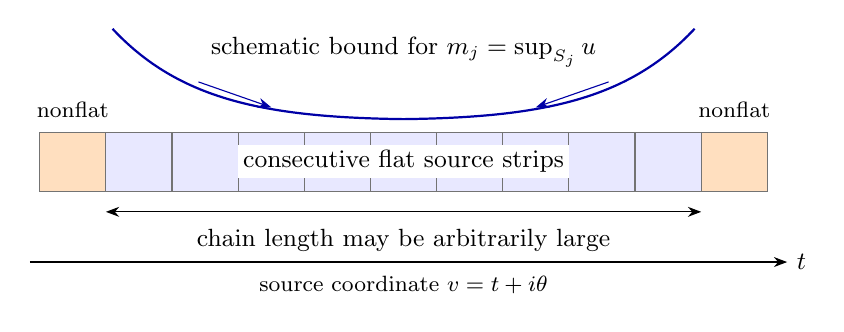
\begin{tikzpicture}[x=0.84cm,y=0.75cm,>=Stealth,
  every node/.style={font=\small}]
 \fill[orange!25] (0,0) rectangle (1,1);
 \fill[blue!9] (1,0) rectangle (10,1);
 \fill[orange!25] (10,0) rectangle (11,1);
 \foreach \x in {0,...,11} {\draw[black!55] (\x,0)--(\x,1);}
 \draw[black!55] (0,0) rectangle (11,1);
 \node[anchor=south,font=\footnotesize] at (0.5,1.08) {nonflat};
 \node[anchor=south,font=\footnotesize] at (10.5,1.08) {nonflat};
 \node[fill=white,inner sep=2pt] at (5.5,0.5)
   {consecutive flat source strips};
 \draw[blue!65!black,thick]
   (1.1,2.75) .. controls (2.1,1.55) and (3.4,1.25) .. (5.5,1.22)
   .. controls (7.6,1.25) and (8.9,1.55) .. (9.9,2.75);
 \node[fill=white,inner sep=2pt] at (5.5,2.35)
   {schematic bound for $m_j=\sup_{S_j}u$};
 \draw[->,blue!65!black] (2.4,1.85)--(3.5,1.42);
 \draw[->,blue!65!black] (8.6,1.85)--(7.5,1.42);
 \draw[<->] (1,-0.35)--(10,-0.35);
 \node[anchor=north] at (5.5,-0.48) {chain length may be arbitrarily large};
 \draw[->] (-0.15,-1.2)--(11.3,-1.2)
   node[anchor=west] {$t$};
 \node[anchor=north,font=\footnotesize] at (5.5,-1.28)
   {source coordinate $v=t+i\theta$};
\end{tikzpicture}
\caption{A flat chain in the source cylinder. The absence of a constant
angular mode makes derivative bounds decay away from the chain's ends.
Their sum, and hence the variation of target height along the chain,
is bounded independently of its length. A chain meeting a target height
slab can therefore be charged to a neighboring nonflat strip in a
fixed enlarged slab. The horizontal coordinate is the source
coordinate $t$, not the target height $h\circ f$.}
\label{fig:flat-chain}
\end{figure}


\begin{proposition}[The cylinder estimate on a target height slab]
\label{cylinder:estimate}
There are constants $R_0,C_0>0$ depending only on the lifted geometry
with the following property.  Let $f:\Omega\to Y$ be a nonconstant
proper holomorphic map from a domain in $\mathcal C$.  Let $w\geq0$
be measurable and suppose
\[
 M_w:=\sup_{j\in\ZZ}\|w\|_{L^2(\Omega\cap S_j)}<\infty.
\]
For every interval $I$ of length one, set
\[
 E_I=\int_{\Omega\cap(h\circ f)^{-1}(I+[-R_0,R_0])}
                          u^2\,dA_v.
\]
If $E_I<\infty$, then
\begin{equation}\label{cylinder:estimate-formula}
 \int_{\Omega\cap(h\circ f)^{-1}(I)}u\,w\,dA_v
            \leq C_0M_w(1+E_I).
\end{equation}
The same estimate holds on a full source half-cylinder cut from a
proper normalization map; properness is used only on thickened strips
away from the artificial initial boundary, and a fixed finite initial
block of strips is included in the constant. The integral on the left is
always restricted to the inverse image of the target interval $I$.
\end{proposition}

\begin{proof}
Take $R_0=\Lambda+\delta$, with constants from the two preceding
lemmas.  Let $\mathcal N_I$ be the set of nonflat strips containing
a point of height in $I+[-\Lambda,\Lambda]$.  The source cylinders
$C_j^Q$ have overlap at most $2Q+3$.  Summing
\eqref{cylinder:energy-cost} over any finite subset of
$\mathcal N_I$ gives
\begin{equation}\label{cylinder:nonflat-count}
 \#\mathcal N_I\leq(2Q+3)\varepsilon_0^{-1}E_I.
\end{equation}
This also proves that the set being counted is finite.  In particular,
the set $\mathcal N'_I$ of nonflat strips hitting $I$ has this bound.
Cauchy--Schwarz, first on each strip restricted to the target slab and
then on the finite sum, gives
\[
 \begin{split}
 &\sum_{j\in\mathcal N'_I}
       \int_{\Omega\cap S_j\cap(h\circ f)^{-1}(I)}u\,w\,dA_v\\
 &\qquad\leq
 M_w(\#\mathcal N'_I)^{1/2}
 \left(\sum_{j\in\mathcal N'_I}
       \int_{\Omega\cap S_j\cap(h\circ f)^{-1}(I)}u^2dA_v\right)^{1/2}
 \leq C M_w E_I.
 \end{split}
\]
Only the intervals appearing explicitly in these integrals are used;
no estimate of the energy outside the enlarged target interval is
being assumed.

On one flat chain, \eqref{cylinder:chain-sum} and
$\|w\|_{L^1(S_j)}\leq\sqrt{2\pi}M_w$ give
\[
 \sum_{j\in J}\int_{S_j}u\,w\,dA_v
      \leq\sqrt{2\pi}M_wL_0.
\]
Every chain meeting $I$ has a finite endpoint adjacent to a member
of $\mathcal N_I$, by Lemma~\ref{cylinder:flat-chains}.
Each nonflat strip has at most two adjacent chains.  Thus at most
$2\#\mathcal N_I$ chains contribute, and their integral over the target
slab is bounded by their full chain integrals. Combining this bound
with \eqref{cylinder:nonflat-count} proves
\eqref{cylinder:estimate-formula} on the full cylinder.

For a half-cylinder, omit the fixed finite block of at most $2Q+4$
strips on which the small-energy neighborhoods meet its initial
boundary.  On this block Cauchy--Schwarz gives
$CM_wE_I^{1/2}\leq CM_w(1+E_I)$.  Apply the preceding argument to the
remaining indices.  There is at most one chain reaching the new
finite endpoint, and its integral is at most
$\sqrt{2\pi}M_wL_0$.  All other chains are charged as before.
Increasing $C_0$ proves the half-cylinder assertion.
\end{proof}

For a proper normalization the integral in \eqref{cylinder:energy}
counts the area of the reduced curve once, away from its discrete
singular set.  A fixed enlargement of a height interval is covered
by a fixed finite number of unit height intervals.  Consequently
\eqref{cylinder:area-input} and Proposition~\ref{cylinder:estimate}
imply, with the same exponent $A$,
\begin{equation}\label{cylinder:exponential}
 \int_{(h\circ f)^{-1}([-\ell-1,-\ell])}u\,w\,dA_v
          \leq C_{B,w}e^{A\ell}\qquad(\ell\in\NN).
\end{equation}
On a half-cylinder the integral is also restricted to that end.
Finitely many height intervals outside the range where the area
estimate was initially proved change only the constant.

\subsection{Excluding nonplane normalizations}

We first apply the estimate with the constant multiplier $w=1$.
This supplies a differential with controlled current mass whenever
the planar normalization omits at least two points of the sphere.

\begin{corollary}\label{cylinder:plane}
If a component of $D$ is noncompact, its normalization is biholomorphic
to $\CC$.
\end{corollary}

\begin{proof}
By Proposition~\ref{curve:genus}, the normalization $R$ is a domain in
$\PP^1$.  If it omits two distinct points, send them by a M\"obius
transformation to $0$ and $\infty$.  Then $R\subset\CC^*$ is a domain
in the logarithmic cylinder and
$\alpha=dz/z=dv$ is a globally defined nonzero holomorphic
differential on $R$.  Formula~\eqref{cylinder:exponential} with
$w=1$ bounds the mass of $f_*\alpha$ on every unit height interval by
$C_Be^{A\ell}$: pulling back a test one-form of norm at most one
costs at most a fixed multiple of $u$, while $|dv|$ is constant.
The scalar case of Proposition~\ref{curve:residue} forbids this
nonzero differential.  Thus $\PP^1\setminus R$ has at most one point.
It has at least one point because $R$ is noncompact.  Removing that
single point gives $R\simeq\CC$.
\end{proof}

\subsection{Excluding plane normalizations}

The scalar residue test leaves only plane normalizations. On a
translated plane the differential $dz$ has an exponentially growing
coefficient in the logarithmic coordinate. We multiply it by the
section of $E$ that tends to zero at the negative end. To control the
product, we first solve the pulled-back Dolbeault equation in a periodic
gauge whose exponential factors have bounded $L^2$ norms on source
strips. The next lemma supplies this gauge, including its angular
constant mode. Its input $a$ is an ordinary complex-valued function;
in the application it will be the coefficient of the pulled-back
connection.

\begin{lemma}[A periodic gauge on the cylinder]
\label{cylinder:gauge}
If $a\in L^1(\mathcal C)\cap L^2(\mathcal C)$, there is a periodic
distribution $g$ satisfying
\[
 \tfrac12(\partial_t+i\partial_\theta)g=a,
 \qquad
 \sup_{j\in\ZZ}\|g\|_{W^{1,2}(S_j)}
       \leq C\bigl(\|a\|_{L^1}+\|a\|_{L^2}\bigr).
\]
For every $p<\infty$ this solution satisfies
\begin{equation}\label{cylinder:gauge-exp}
 \sup_j\int_{S_j}\exp\bigl(p|\operatorname{Re}g|\bigr)dA_v<\infty.
\end{equation}
If $a$ is smooth in an open set, $g$ is smooth there.
\end{lemma}

\begin{proof}
Let $a_0(t)=(2\pi)^{-1}\int_0^{2\pi}a(t,\theta)d\theta$.
Its primitive
\[
 g_0(t)=2\int_{-\infty}^t a_0(s)ds
\]
is bounded by $\pi^{-1}\|a\|_{L^1}$, and
$g_0'=2a_0\in L^2(\RR)$.  This bounds its full $W^{1,2}$ norm on
each unit strip, including its mean.  For $a_\perp=a-a_0$, take
Fourier series in $\theta$ and Fourier transform in $t$.  For every
integer $n\ne0$ define
\[
 \widehat{g_\perp}(\xi,n)
       =\frac{2\widehat{a_\perp}(\xi,n)}{i\xi-n}.
\]
Since $|n|\geq1$, each of the multipliers
$1/(i\xi-n)$, $\xi/(i\xi-n)$, and $n/(i\xi-n)$ is bounded in
absolute value by one.  Plancherel therefore gives
$\|g_\perp\|_{W^{1,2}(\mathcal C)}\leq C\|a\|_{L^2}$.
The sum $g=g_0+g_\perp$ has the asserted periodicity, equation, and
stripwise bound.  Local elliptic regularity for
$\partial_t+i\partial_\theta$ gives the last assertion.

Let $B$ be a uniform bound for these stripwise norms.  The
two-dimensional Trudinger inequality on a fixed bounded strip
\cite{Trudinger1967}, including the $L^2$ term in the norm, gives
constants $c,C>0$ independent of $j$ such that
\[
 \int_{S_j}\exp\left(\frac{c|\operatorname{Re}g|^2}{B^2}\right)dA_v
       \leq C
\]
when $B>0$.  One can cut the cylinder at a fixed angle and apply the
bounded-rectangle form of that inequality; no boundary value of $g$
is prescribed.  The zero-norm case is immediate.  For each finite
$p$, the inequality
$p|x|\leq cx^2/B^2+p^2B^2/(4c)$ proves
\eqref{cylinder:gauge-exp}.  In particular both
$e^{\operatorname{Re}g}$ and $e^{-\operatorname{Re}g}$ have bounded
$L^p$ norms on unit strips, for every fixed finite $p$.
\end{proof}

\begin{theorem}\label{cylinder:compactness}
Every irreducible component of $D$ is compact and has rational
normalization.
\end{theorem}

\begin{proof}
It remains, by Proposition~\ref{curve:genus} and
Corollary~\ref{cylinder:plane}, to exclude a component with proper
normalization $f:\CC\to B\subset Y$.  Let
$M_B=\sup_Bh<\infty$ and $M_D=\sup_Dh<\infty$.
The curves $B_k=T^kB$ are distinct, since their height suprema are
$M_B+k$.  For every sufficiently large positive integer $k$ this
supremum exceeds $M_D$, so $B_k$ is not contained in $D$.
Write $f_k=T^k\circ f$.  We will construct on each of these curves
the nonzero $f_k^*E$-valued holomorphic differential
\begin{equation}\label{cylinder:bundle-differential}
 \alpha_k=(f_k^*s)\,dz
\end{equation}
and prove that its pushforward has growth exponent $A$.

The key point is the cancellation of the growth of $dz$. Properness
sends the exterior of the plane to the negative end of $Y$. After a
periodic change of frame there, the section coefficient becomes an
ordinary holomorphic function tending to zero at infinity, hence of
size $O(1/|z|)$. Since $dz=z\,dv$, this leaves only an exponential
gauge factor, whose stripwise $L^2$ bound is exactly the multiplier
hypothesis in Proposition~\ref{cylinder:estimate}.

Fix one such $k$ temporarily.  Properness, together with the upper
height bound, implies
\begin{equation}\label{cylinder:proper-end}
 h(f_k(z))\longrightarrow-\infty
                  \quad\hbox{uniformly as }|z|\longrightarrow\infty.
\end{equation}
Indeed, otherwise a sequence with $|z|\to\infty$ would have image in
some compact height slab $\{c\leq h\leq M_B+k\}$, contradicting
properness.  On an exterior disk $|z|>R_k$ we may therefore use the
prescribed smooth negative-end frame of $E$.  Choose its Hermitian
norm to be one on that end.  In this frame write
$\dbar_E=\dbar+\eta$, where
$|\eta|\leq C e^{-\gamma|h|}$; this is the choice
\eqref{curve:gamma-choice}.  In the logarithmic coordinate $v=\log z$,
write $f_k^*\eta=a(v)d\bar v$.  Then
\begin{equation}\label{cylinder:connection-bound}
 |a(v)|\leq C e^{-\gamma|h(f_k(v))|}\,u(v).
\end{equation}

After increasing $R_k$, the entire image of this exterior disk has
negative height.  Summing \eqref{cylinder:connection-bound} over its
target height intervals, using \eqref{cylinder:exponential} with
$w=1$ for the first estimate and \eqref{cylinder:energy} for the
second, gives
\begin{align*}
 \int |a|\,dA_v
   &\leq C_k\sum_{\ell\geq0}e^{-(\gamma-A)\ell}<\infty,\\
 \int |a|^2\,dA_v
   &\leq C_k\sum_{\ell\geq0}e^{-(2\gamma-A)\ell}<\infty.
\end{align*}
An initial compact annulus only adds a finite quantity.  Smoothly
cut $a$ off toward the finite side and extend by zero to the full
cylinder.  This retains both bounds and agrees with $a$ on a
slightly smaller exterior disk.  Lemma~\ref{cylinder:gauge} gives
a single-valued periodic smooth gauge $g$ there, with
$\dbar g=a\,d\bar v$ and uniformly bounded stripwise
$W^{1,2}$ norms.

Let $\sigma(v)$ be the coefficient of $f_k^*s$ in the same smooth
frame.  Holomorphicity says $\dbar\sigma+a\sigma\,d\bar v=0$.
Hence
\[
 H(v)=e^{g(v)}\sigma(v)
\]
is ordinary holomorphic and periodic on the exterior cylinder.
By Proposition~\ref{compact:section} and \eqref{cylinder:proper-end},
$\sup_{S_j}|\sigma|\to0$ as $j\to\infty$.  The exponential
estimate \eqref{cylinder:gauge-exp} therefore yields
\[
 \int_{S_j}|H|^2dA_v
 \leq\left(\sup_{S_j}|\sigma|^2\right)
                    \int_{S_j}e^{2\operatorname{Re}g}dA_v
       \longrightarrow0.
\]
The mean-value inequality on fixed small disks in the cylinder,
each contained in the union of three adjacent strips, implies
$H(v)\to0$ uniformly as $t\to\infty$.  Viewed as a holomorphic
function of $z$, it consequently extends holomorphically across
$z=\infty$ with value zero.  Its Taylor expansion in $1/z$ gives
\begin{equation}\label{cylinder:H-decay}
 |H(z)|\leq C_k|z|^{-1}
\end{equation}
on a further exterior disk.

Since $dz=e^v\,dv$, Equations \eqref{cylinder:bundle-differential}
and \eqref{cylinder:H-decay} give the coefficient estimate
\[
 |\alpha_k|_v=|e^v\sigma(v)|
        \leq C_k e^{-\operatorname{Re}g(v)}.
\]
Here $|\cdot|_v$ is the norm of its coefficient relative to $dv$
and the unit smooth frame.  The right-hand factor has uniformly
bounded $L^2$ norms on unit strips by
\eqref{cylinder:gauge-exp}.  Apply
\eqref{cylinder:exponential} with
$w=e^{-\operatorname{Re}g}$.  Pullback of a test one-form costs at
most $Cu$, so this proves
\begin{equation}\label{cylinder:current-growth}
 \Mass\left((f_k)_*\alpha_k\bigm|_{h^{-1}([-\ell-1,-\ell])}\right)
          \leq C_k'e^{A\ell}\qquad(\ell\geq0).
\end{equation}
The omitted compact disk in the source has compact image and
contributes only on finitely many height intervals, which are
absorbed in $C_k'$.  The section $f_k^*s$ is nonzero because
$B_k\not\subset D$, and $dz$ is nowhere zero; thus $\alpha_k$ is a
nonzero holomorphic bundle-valued differential.

Finally fix, once and for all, an admissible $\eps>0$ and a number
$b>\max\{A,\eps\}$.  The currents in
\eqref{cylinder:current-growth} all belong to the same degree-one
space $W^{-4}_{-\eps,b}$ of the shifted complex from
Theorem~\ref{weighted:currents}; their coefficients take values
in the same bundle $E$.  Their positive supports are bounded
separately, and any finite collection has a common upper support
bound.  Proposition~\ref{curve:residue} therefore makes the classes
of every finite collection linearly independent in the single
space $H^{2,1}_{-\eps,b}(Y,E)$.  That space is finite dimensional
by Theorem~\ref{weighted:currents}.  Infinitely many distinct
$B_k$ contradict this finite dimension.  The constants $C_k'$ may
vary; no bound on their supremum has been used.  The exponent $A$,
the weights, and the Sobolev orders were fixed throughout.
This excludes the plane case and completes the proof.
\end{proof}

\section{Counting rational curves and obtaining the shell}
\label{sec:conclusion}

We apply the preceding analysis to every datum of
Lemma~\ref{compact:classes}, using the decay rate fixed after
Lemma~\ref{curve:area}. Proposition~\ref{compact:section} gives a divisor
$D_i$ with ordinary class $j(e_i)$. By
Theorem~\ref{cylinder:compactness}, every irreducible component of
$D_i$ is compact and has rational normalization. The divisor as a whole
may still have infinitely many components; it is locally finite and
bounded above in height. This distinction will be retained in all
intersection pairings below.

\begin{lemma}[Lifts of rational curves]\label{conclusion:lifts}
Every compact rational curve in $Y$ projects to a rational curve in $X$.
For each rational curve $B\subset X$, the compact irreducible curves in
$Y$ projecting onto $B$ form one orbit under $T$. In particular, a
collection of $r$ rational curves in $X$ gives at most $nr$ orbits of
compact lifts under $S=T^n$.
\end{lemma}

\begin{proof}
The image under $\pi$ of a compact curve is a compact analytic curve,
because the map restricted to that curve is proper and locally finite.
It is nonconstant since $\pi$ is a local biholomorphism. If the upstairs
normalization is $\PP^1$, the induced nonconstant map to the normalization
of the image is a finite map from $\PP^1$ to a compact Riemann surface.
Riemann--Hurwitz forces that surface to have genus zero. Thus the image
is rational.

Conversely, let $\nu:\PP^1\to B\subset X$ be the normalization of a
rational curve. Since $\PP^1$ is simply connected, the map $\nu$ lifts
to a holomorphic map $\widetilde\nu:\PP^1\to Y$ after a choice of the
image of one point. Its image $\widetilde B$ is compact and irreducible.
Over the smooth part of $B$, its projection has degree one, because
$\nu$ does. The lifts of this fixed normalization map form one orbit
under the deck group, so their images do also.

To see that these are all the compact irreducible curves over $B$, take
such a curve $C$ and a point of it over the smooth part of $B$.
Choose the lift of $\nu$ through this point. The local biholomorphism
property of $\pi$ makes its image and $C$ agree in a nonempty open
curve germ. Irreducibility and analytic continuation then make their
images equal. This proves the orbit assertion. Splitting the integer
deck powers into their $n$ residue classes proves the bound for $S$.

This argument lifts the normalization map, not the singular topological
space $B$. In particular it also applies to a nodal rational curve;
the connected components of its full inverse image need not be compact.
\end{proof}

One curve downstairs accounts for infinitely many translates upstairs.
We therefore count independent compact classes over a ring in which
multiplication by $t$ records one deck translation. A single orbit of
compact curves will then impose one linear equation over the fraction
field of that ring. The intersection pairing will show that fewer curve
orbits than independent classes are impossible.

Fix $n$, put $S=T^n$, and set
\[
 \Lambda=\mathbb Q[t,t^{-1}],\qquad
 \mathbb F=\mathbb Q(t),\qquad \overline{f(t)}=f(t^{-1}).
\]
On compactly supported cohomology, let
\[
 ta=S_!a:=(S^{-1})^*a.
\]
This is the convention that translates the support in the positive
$S$-direction. It agrees with the pushforward action $C\mapsto S_*C$
on homology under Poincar\'e duality. Define
\begin{equation}\label{conclusion:laurent-pairing}
 P(a,b)=\sum_{k\in\ZZ}\langle a,S_!^k b\rangle t^k
 \quad(a,b\in H_c^2(Y;\mathbb Q)).
\end{equation}
This is a Laurent polynomial: compactly supported representatives
intersect only finitely many translates of one another. Invariance of
intersection under $S$ and symmetry in degree two give
\begin{equation}\label{conclusion:sesquilinearity}
 P(ta,b)=tP(a,b),\qquad P(a,tb)=t^{-1}P(a,b),\qquad
 P(b,a)=\overline{P(a,b)}.
\end{equation}
Thus $P$ is linear in its first variable and conjugate-linear in its
second, where conjugation means only the involution $t\mapsto t^{-1}$.
For a compact oriented curve $C$, define similarly
\begin{equation}\label{conclusion:curve-pairing}
 Q(a,C)=\sum_{k\in\ZZ}\left(\int_{S_*^k C}a\right)t^k.
\end{equation}
This is finite and $\Lambda$-linear in $a$ with the same convention.
Its vanishing is equivalent to the vanishing of the ordinary pairing
of $a$ with every $S$-translate of $C$.

\begin{lemma}[Nonsingularity of the compact classes]
\label{conclusion:pairing-rank}
For the classes $e_1,\ldots,e_d$ of Lemma~\ref{compact:classes}, the
matrix $P(t)=(P(e_i,e_j))_{i,j=1}^d$ has nonzero determinant in
$\Lambda$. Their $\Lambda$-span is free of rank $d$, and $P$ is
nonsingular on its extension of scalars to $\mathbb F$.
\end{lemma}

\begin{proof}
Let $w_i$ be the transferred classes in $X_n$. Periodizing compactly
supported closed representatives of $e_i$ and $e_j$, then integrating
over one fundamental period, gives
\begin{equation}\label{conclusion:evaluation-one}
 P(e_i,e_j)(1)
 =\sum_{k\in\ZZ}\langle e_i,S_!^k e_j\rangle
 =w_i\cdot w_j.
\end{equation}
For completeness, the periodization is the locally finite sum of all
$S_!$-translates of a representative; it descends to a closed form on
$X_n$. In the integral of the wedge product of two such sums, change
variables by the translate in the first factor. The translated
fundamental periods tile $Y$, leaving the displayed sum indexed by the
relative translate of the second factor. Compact supports justify
every interchange. In the construction of Lemma~\ref{compact:classes}
the forms are supported inside the same open period, so terms with
$k\neq0$ actually vanish; the periodization identity also records the
intrinsic pairing convention.

The classes $w_i$ are independent over $\mathbb Q$ and the form on
$X_n$ is negative definite. Their Gram matrix is therefore negative
definite, in particular invertible. Equation~\eqref{conclusion:evaluation-one}
implies $\det P(1)\neq0$, so $\det P(t)$ is not the zero Laurent
polynomial. The matrix is invertible over $\mathbb F$.
If $\sum_i f_i(t)e_i=0$ for $f_i\in\Lambda$, pairing with each $e_j$
and using \eqref{conclusion:sesquilinearity} gives
$(f_1,\ldots,f_d)P(t)=0$. Invertibility over $\mathbb F$ forces every
$f_i=0$. This proves freeness and the asserted nonsingularity.
\end{proof}

\begin{proposition}[The required number of rational curves]
\label{conclusion:curves}
The surface $X$ contains at least $b_2(X)$ rational curves.
\end{proposition}

\begin{proof}
If there are infinitely many, the conclusion is immediate. Otherwise
suppose for a contradiction that their number is $r<b_2(X)$, and list
all of them. Choose $n$ so large that
\[
 n\bigl(b_2(X)-r\bigr)>C_0.
\]
Lemma~\ref{compact:classes} then gives $d>nr$ compact classes.
By Lemma~\ref{conclusion:lifts}, choose representatives
$C_1,\ldots,C_q$ for all $S$-orbits of compact irreducible lifts of the
listed rational curves, where $q\leq nr<d$.

Consider over $\mathbb F$ the $q$ homogeneous linear equations
\begin{equation}\label{conclusion:annihilating-equations}
 \sum_{i=1}^d f_i(t)\,Q(e_i,C_\ell)=0,
 \qquad 1\leq\ell\leq q.
\end{equation}
There are more unknowns than equations, so a nonzero solution exists.
Multiplying all its entries by a common nonzero denominator gives
$f_i\in\Lambda$, not all zero. The compactly supported class
\[
 x=\sum_{i=1}^d f_i(t)e_i
\]
is nonzero by Lemma~\ref{conclusion:pairing-rank}; its support is compact
because this is a finite Laurent combination. Equations
\eqref{conclusion:annihilating-equations} and
\eqref{conclusion:curve-pairing} imply that $x$ pairs to zero with
every compact rational lift and every one of its $S$-translates.

For each $j$, the ordinary class $j(e_j)$ is represented by the divisor
$D_j$. Every component of $D_j$ is compact rational by
Theorem~\ref{cylinder:compactness}, and its image downstairs is rational
by Lemma~\ref{conclusion:lifts}. Hence each component occurs among the
curves just annihilated by $x$. If $\alpha$ is a compactly supported
closed real two-form representing $x$, the ordinary divisor identity
\eqref{compact:divisor-pairing} gives, for every $k\in\ZZ$,
\[
 \langle x,S_!^k e_j\rangle
 =\int_{S_*^kD_j}\alpha=0.
\]
Indeed local finiteness makes the last integral a finite sum of
integrals over compact components meeting $\supp\alpha$, and each
summand is zero by the curve orthogonality. This argument pairs a
compact test class with a locally finite divisor; it never pairs two
locally finite cycles or sums an infinite Laurent series.

We have proved $P(x,e_j)=0$ for all $j$. By
\eqref{conclusion:sesquilinearity} this says
$(f_1,\ldots,f_d)P(t)=0$, contradicting the nonsingularity of $P(t)$
over $\mathbb F$. Therefore $r\geq b_2(X)$.
\end{proof}

\begin{lemma}[Independence of curve classes]
\label{conclusion:upper-bound}
Under \eqref{surface:no-square-zero}, the real cohomology classes of
any finite collection of distinct curves on $X$ are linearly
independent. Consequently $X$ has at most $b_2(X)$ curves in total.
\end{lemma}

\begin{proof}
Suppose a finite collection admits a nonzero real relation. Split its
positive and negative coefficients to obtain effective real divisors
$A$ and $B$ with disjoint lists of components and $[A]=[B]=v$; one of
them may be empty. If $v\neq0$, both are nonempty and negative
definiteness gives $v^2<0$. But positivity of local intersections of
distinct complex curves gives
\[
 v^2=A\cdot B\geq0,
\]
a contradiction. Thus $v=0$. At least one nonempty effective real
divisor, say $A=\sum_{i\in I}a_i B_i$ with all $a_i>0$, has zero real
class.

To pass from this real relation to an integral one, express the classes
$[B_i]$ in an integral basis of $H^2(X;\ZZ)/\operatorname{Tors}$.
The relation space is the kernel of an integer matrix, hence has a
basis over $\mathbb Q$. Its rational points are dense in its real
points. Approximate $(a_i)_{i\in I}$ within this kernel by a rational
vector with all coordinates still positive, and clear denominators.
The result is a nonzero effective integral divisor with zero real
class and hence square zero. This contradicts
\eqref{surface:no-square-zero}. There is no relation. Since
$\dim H^2(X;\RR)=b_2(X)$, any collection of more than $b_2(X)$ curves
would contain such a finite dependent collection.
\end{proof}

\begin{proof}[Proof of Theorem~\ref{thm:main}]
If $X$ has a nonzero effective square-zero divisor,
Proposition~\ref{surface:reduction}\textup{(i)} already gives the
desired shell. In the remaining case,
Proposition~\ref{conclusion:curves} and
Lemma~\ref{conclusion:upper-bound} show that $X$ has exactly $b_2(X)$
rational curves. It is compact and minimal, has $b_1(X)=1$,
$\kappa(X)=-\infty$, and $b_2(X)>0$ by the original hypotheses.
Every hypothesis of the Main Theorem of Dloussky--Oeljeklaus--Toma is
therefore satisfied, so Proposition~\ref{surface:reduction}\textup{(ii)}
applies.

The conclusion in \cite[pp.~283--284]{DOT2003} is an open neighborhood
$U$ of the unit sphere in $\CC^2\setminus\{0\}$ and a biholomorphism
$\phi:U\to\Sigma\subset X$ such that $X\setminus\Sigma$ is connected.
This is precisely the conclusion required in Theorem~\ref{thm:main}.
Equivalently, if a shell is described by its nonseparating core sphere,
choose a sufficiently small round annular collar in the given
holomorphic neighborhood. On either side of the core, the collar
coordinate pushes the complement of the core onto the complement of
the smaller open collar. The latter is therefore connected as well.
\end{proof}

\subsection{Consequences of the shell}\label{sec:consequences}

The shell now gives the deformation and topological description stated
in the introduction, and removes the remaining class VII exception in
the aspherical-surface inequality.

\begin{proof}[Proof of Corollary~\ref{cor:topology}]
Theorem~\ref{thm:main} supplies a global spherical shell. Kato's
deformation theorem \cite[Theorem~1]{Kato1977} then gives a
one-parameter deformation with each nonzero fiber a modification of a
primary Hopf surface; his Corollary~1 gives $\pi_1(X)\cong\ZZ$.
In complex dimension two, a modification between smooth surfaces factors
as a finite succession of point blowups, with possibly infinitely near
centers \cite{BHPV2004}.

After shrinking $\Delta$, the family is a proper smooth submersion.
Ehresmann's theorem identifies its fibers by diffeomorphisms preserving
their continuously varying complex orientations. Every primary Hopf
surface is diffeomorphic to $S^1\times S^3$
\cite[\S1, p.~1109]{GauduchonOrnea1998}, and hence has second Betti number
zero. Each complex point blowup increases the second Betti number by one
and replaces the oriented smooth manifold by its connected sum with
$\overline{\mathbb{CP}}^{\,2}$ \cite{BHPV2004}. Since the fibers have
second Betti number $b$, there are exactly $b$ blowups, and the asserted
oriented smooth type follows. The product orientation can be chosen
compatibly because $S^1\times S^3$ admits an orientation-reversing
diffeomorphism.
\end{proof}

\begin{proof}[Proof of Corollary~\ref{cor:aspherical-geography}]
Albanese--Di Cerbo--Lombardi~\cite[Theorem~1.4]{AlbaneseDiCerboLombardi2025}
prove these conclusions except for the possible case of a class
$\mathrm{VII}_0^+$ surface violating the Global Spherical Shell conjecture.
Theorem~\ref{thm:main} excludes that case. Corollary~\ref{cor:topology}
also explains the non-asphericity: such a surface has $\pi_1\cong\ZZ$
and $b_2>0$, but an aspherical manifold with fundamental group $\ZZ$
is homotopy equivalent to $S^1$.
\end{proof}

\begin{thebibliography}{99}

\bibitem{AlbaneseDiCerboLombardi2025}
M.~Albanese, L.~F. Di Cerbo, and L.~Lombardi,
Aspherical complex surfaces, the Singer conjecture, and Gromov--L\"uck
inequality $\chi\geq|\sigma|$,
\emph{Math. Proc. Cambridge Philos. Soc.} \textbf{179} (2025), 541--555.
\href{https://doi.org/10.1017/S0305004125101400}{doi:10.1017/S0305004125101400}.
Author version: arXiv:2311.10226v4, 21 July 2025.
\href{https://arxiv.org/abs/2311.10226v4}{arXiv:2311.10226v4}.

\bibitem{AtiyahSingerIII1968}
M.~F. Atiyah and I.~M. Singer, The index of elliptic operators. III,
\emph{Ann. of Math. (2)} \textbf{87} (1968), no.~3, 546--604.
\href{https://doi.org/10.2307/1970717}{doi:10.2307/1970717}.

\bibitem{BHPV2004}
W.~P. Barth, K.~Hulek, C.~A.~M. Peters, and A.~Van de Ven,
\emph{Compact Complex Surfaces}, second enlarged edition,
Ergebnisse der Mathematik und ihrer Grenzgebiete, 3.~Folge, vol.~4,
Springer-Verlag, Berlin, 2004.
\href{https://doi.org/10.1007/978-3-642-57739-0}{doi:10.1007/978-3-642-57739-0}.

\bibitem{Bishop1964}
E.~Bishop, Conditions for the analyticity of certain sets,
\emph{Michigan Math. J.} \textbf{11} (1964), no.~4, 289--304.
\href{https://doi.org/10.1307/mmj/1028999180}{doi:10.1307/mmj/1028999180}.

\bibitem{Bogomolov1976}
F.~A. Bogomolov, Classification of surfaces of class $\mathrm{VII}_0$
with $b_2=0$, \emph{Math. USSR-Izv.} \textbf{10} (1976), no.~2, 255--269.
\href{https://doi.org/10.1070/IM1976v010n02ABEH001688}{doi:10.1070/IM1976v010n02ABEH001688}.

\bibitem{Buchdahl1999}
N.~Buchdahl, On compact K\"ahler surfaces,
\emph{Ann. Inst. Fourier (Grenoble)} \textbf{49} (1999), no.~1, 287--302.
\href{https://doi.org/10.5802/aif.1674}{doi:10.5802/aif.1674}.

\bibitem{Demailly2012}
J.-P. Demailly, \emph{Complex Analytic and Differential Geometry},
author manuscript, 21 June 2012.
\href{https://www-fourier.univ-grenoble-alpes.fr/~demailly/manuscripts/agbook.pdf}{Author PDF}.

\bibitem{Dloussky1984}
G.~Dloussky, \emph{Structure des surfaces de Kato},
M\'em. Soc. Math. France (N.S.), no.~14 (1984), ii+120 pp.
\href{https://doi.org/10.24033/msmf.297}{doi:10.24033/msmf.297}.

\bibitem{Dloussky2006}
G.~Dloussky, On surfaces of class $\mathrm{VII}_0^+$ with numerically
anticanonical divisor, \emph{Amer. J. Math.} \textbf{128} (2006),
no.~3, 639--670.
\href{https://doi.org/10.1353/ajm.2006.0021}{doi:10.1353/ajm.2006.0021}.

\bibitem{Dloussky2025}
G.~Dloussky, On classification of compact complex surfaces of class VII,
in \emph{Real and Complex Geometry: In Honour of Paul Gauduchon},
L.~Ornea (ed.), Springer, Cham, 2025, pp.~159--189.
\href{https://doi.org/10.1007/978-3-031-92297-8_7}{doi:10.1007/978-3-031-92297-8\_7}.
Revised author version: arXiv:2403.20178v2, 21 December 2025.
\href{https://arxiv.org/abs/2403.20178v2}{arXiv:2403.20178v2}.

\bibitem{DOT2003}
G.~Dloussky, K.~Oeljeklaus, and M.~Toma,
Class $\mathrm{VII}_0$ surfaces with $b_2$ curves,
\emph{Tohoku Math. J. (2)} \textbf{55} (2003), no.~2, 283--309.
\href{https://doi.org/10.2748/tmj/1113246942}{doi:10.2748/tmj/1113246942}.

\bibitem{DlousskyTeleman2012}
G.~Dloussky and A.~Teleman, Infinite bubbling in non-K\"ahlerian geometry,
\emph{Math. Ann.} \textbf{353} (2012), no.~4, 1283--1314.
\href{https://doi.org/10.1007/s00208-011-0713-9}{doi:10.1007/s00208-011-0713-9}.

\bibitem{Donaldson1987}
S.~K. Donaldson, The orientation of Yang--Mills moduli spaces and
$4$-manifold topology,
\emph{J. Differential Geom.} \textbf{26} (1987), no.~3, 397--428.
\href{https://doi.org/10.4310/jdg/1214441485}{doi:10.4310/jdg/1214441485}.

\bibitem{Enoki1981}
I.~Enoki, Surfaces of class $\mathrm{VII}_0$ with curves,
\emph{Tohoku Math. J. (2)} \textbf{33} (1981), no.~4, 453--492.
\href{https://doi.org/10.2748/tmj/1178229349}{doi:10.2748/tmj/1178229349}.

\bibitem{Gauduchon1977}
P.~Gauduchon, Le th\'eor\`eme de l'excentricit\'e nulle,
\emph{C. R. Acad. Sci. Paris S\'er. A--B} \textbf{285} (1977), A387--A390.

\bibitem{GauduchonOrnea1998}
P.~Gauduchon and L.~Ornea, Locally conformally K\"ahler metrics on Hopf surfaces,
\emph{Ann. Inst. Fourier (Grenoble)} \textbf{48} (1998), no.~4, 1107--1127.
\href{https://doi.org/10.5802/aif.1651}{doi:10.5802/aif.1651}.

\bibitem{HarveyShiffman1974}
R.~Harvey and B.~Shiffman, A characterization of holomorphic chains,
\emph{Ann. of Math. (2)} \textbf{99} (1974), no.~3, 553--587.
\href{https://doi.org/10.2307/1971062}{doi:10.2307/1971062}.

\bibitem{Hemasundar2011}
G.~V.~V. Hemasundar, Koebe's general uniformisation theorem for
planar Riemann surfaces,
\emph{Ann. Polon. Math.} \textbf{100} (2011), no.~1, 77--85.
\href{https://doi.org/10.4064/ap100-1-7}{doi:10.4064/ap100-1-7}.

\bibitem{Hormander1990}
L.~H\"ormander,
\emph{The Analysis of Linear Partial Differential Operators I:
Distribution Theory and Fourier Analysis}, second edition,
Grundlehren der mathematischen Wissenschaften, vol.~256,
Springer-Verlag, Berlin, 1990.

\bibitem{Kato1977}
Ma.~Kato, Compact complex manifolds containing ``global'' spherical shells,
\emph{Proc. Japan Acad.} \textbf{53} (1977), no.~1, 15--16.
\href{https://doi.org/10.3792/pja/1195517920}{doi:10.3792/pja/1195517920}.

\bibitem{Kodaira1964}
K.~Kodaira, On the structure of compact complex analytic surfaces, I,
\emph{Amer. J. Math.} \textbf{86} (1964), no.~4, 751--798.
\href{https://doi.org/10.2307/2373157}{doi:10.2307/2373157}.

\bibitem{KurnosovSpicer2026}
N.~Kurnosov and C.~Spicer, Class VII surfaces with $b_2=3$ and two
foliations are Kato, arXiv:2608.29047v1, 29 August 2026.
\href{https://arxiv.org/abs/2608.29047v1}{arXiv:2608.29047v1}.

\bibitem{LiYauZheng1994}
J.~Li, S.-T. Yau, and F.~Zheng, On projectively flat Hermitian manifolds,
\emph{Comm. Anal. Geom.} \textbf{2} (1994), no.~1, 103--109.
\href{https://doi.org/10.4310/CAG.1994.v2.n1.a6}{doi:10.4310/CAG.1994.v2.n1.a6}.

\bibitem{MRS2014}
T.~Mrowka, D.~Ruberman, and N.~Saveliev,
Index theory of the de Rham complex on manifolds with periodic ends,
\emph{Algebr. Geom. Topol.} \textbf{14} (2014), no.~6, 3689--3700.
\href{https://doi.org/10.2140/agt.2014.14.3689}{doi:10.2140/agt.2014.14.3689}.

\bibitem{Nakamura1984}
I.~Nakamura, Classification of non-K\"ahler complex surfaces (in Japanese),
\emph{S\^ugaku} \textbf{36} (1984), no.~2, 110--124.
\href{https://doi.org/10.11429/sugaku1947.36.110}{doi:10.11429/sugaku1947.36.110}.

\bibitem{Nakamura1989}
I.~Nakamura, Towards classification of non-K\"ahlerian complex surfaces,
\emph{Sugaku Expositions} \textbf{2} (1989), 209--229.

\bibitem{Taubes1987}
C.~H. Taubes, Gauge theory on asymptotically periodic $4$-manifolds,
\emph{J. Differential Geom.} \textbf{25} (1987), no.~3, 363--430.
\href{https://doi.org/10.4310/jdg/1214440981}{doi:10.4310/jdg/1214440981}.

\bibitem{Teleman1994}
A.-D. Teleman, Projectively flat surfaces and Bogomolov's theorem on
class $\mathrm{VII}_0$ surfaces,
\emph{Internat. J. Math.} \textbf{5} (1994), no.~2, 253--264.
\href{https://doi.org/10.1142/S0129167X94000152}{doi:10.1142/S0129167X94000152}.

\bibitem{Teleman2005}
A.~Teleman, Donaldson theory on non-K\"ahlerian surfaces and class VII
surfaces with $b_2=1$, \emph{Invent. Math.} \textbf{162} (2005), no.~3,
493--521.
\href{https://doi.org/10.1007/s00222-005-0451-2}{doi:10.1007/s00222-005-0451-2}.

\bibitem{Teleman2010}
A.~Teleman, Instantons and curves on class VII surfaces,
\emph{Ann. of Math. (2)} \textbf{172} (2010), no.~3, 1749--1804.
\href{https://doi.org/10.4007/annals.2010.172.1749}{doi:10.4007/annals.2010.172.1749}.

\bibitem{Trudinger1967}
N.~S. Trudinger, On imbeddings into Orlicz spaces and some applications,
\emph{J. Math. Mech.} \textbf{17} (1967), no.~5, 473--483.
\href{https://doi.org/10.1512/iumj.1968.17.17028}{doi:10.1512/iumj.1968.17.17028}.

\end{thebibliography}

\end{document}
